\documentclass{article}
\usepackage{graphicx}
\usepackage{enumitem}

% Settings 
%% Basic information/variables %%
\def\myname{Nong Minh Hieu}
\def\myschool{
    School of Physical and Mathematical Sciences\\
    Nanyang Technological University (NTU - Singapore)
}
\def\subject{Financial Risk Analytics I}

%% Define boolean variables %%
%\newif\issample % Comment when creating a real note
%\newif\showmanual % Comment when creating a real note

\usepackage{tcolorbox}
\usepackage{amssymb}
\tcbuselibrary{theorems}
\usepackage{amsmath,amsthm}
\usepackage{thmtools}
\usepackage[nottoc]{tocbibind}
\usepackage[english]{babel}
\usepackage{xhfill}
\usepackage{changepage}
\usepackage{listings}
\usepackage{xcolor}
\usepackage{framed}
\usepackage{etoolbox}
\usepackage{biblatex} 
\usepackage{fancyhdr}
\usepackage{booktabs}
\usepackage{amsmath}
\usepackage{csquotes}
\usepackage{tikz}
\usepackage{eso-pic}
\usepackage{hyperref}
\usepackage{cleveref}
\addbibresource{main.bib} 

%% Setting up hyperref options %%
\hypersetup{
    colorlinks,
    linkcolor={red!50!black},
    citecolor={blue!50!black},
    urlcolor={blue!80!black}
}

%% Theorem style %%
\newtheoremstyle{definition}
                {5pt} % top space
                {5pt} % bottom space
                {\itshape} % font
                {0pt} % indent
                {\bfseries} % theorem name font
                {. \hrulefill}
                {\newline}
                {\thmname{#1}\thmnumber{ #2}\textnormal{\thmnote{ (#3)}}}

\newenvironment{subproof}[1]
{
    \begin{adjustwidth}{0pt}{}
    \textbf{#1}
    \newline
}
{
    \end{adjustwidth}
}
\newtheoremstyle{proof}
                {10pt} % top space
                {10pt} % bottom space
                {\itshape} % font
                {0pt} % indent
                {\bfseries} % theorem name font
                {. \hrulefill}
                {\newline}
                {\thmname{#1}\thmnumber{ #2}\textnormal{\thmnote{ (#3)}}}

\newtcbtheorem[number within=section, list inside={proplist}]
    {proposition}% name
    {Proposition}% title
    {%
        colback=red!5,
        colframe=red!35!black,
        fonttitle=\bfseries,
    }% options
    {prop}% prefix

\newtcbtheorem[number within=section, list inside={theoremlist}]
    {theorem}% name
    {Theorem}% title
    {%
        colback=blue!5,
        colframe=blue!35!black,
        fonttitle=\bfseries,
    }% options
    {thm}% prefix

\newtcbtheorem[number within=section]
    {lemma}% name
    {Lemma}% title
    {%
        colback=yellow!5,
        colframe=yellow!35!black,
        fonttitle=\bfseries,
    }% options
    {lem} % prefix

\newtcbtheorem[number within=section, list inside={corolist}]
    {corollary}% name
    {Corollary}% title
    {%
        colback=cyan!5,
        colframe=cyan!35!black,
        fonttitle=\bfseries,
    }% options
    {coro} % prefix

%% Proofs %%
\theoremstyle{proof}
\newtheorem*{pf*}{Proof}
\newenvironment{proof*}{
\begin{pf*}
}{
\hfill $\square{}$.
\end{pf*}
}

%% Definitions %%
\theoremstyle{definition}
\declaretheorem[name=Definition, numberwithin=section]{dfn}
\addto\captionsenglish{ \renewcommand{\listtheoremname}{A \ List of Definitions} }
\newenvironment{definition}{\begin{shaded}\begin{dfn}}{\end{dfn}\end{shaded}}
\colorlet{shadecolor}{white!25}

%% Indicator function %%
\DeclareMathAlphabet{\mathmybb}{U}{bbold}{m}{n}
\newcommand{\1}[1]{\mathmybb{1}_{\{#1\}}}

%% Brackets shortcuts %%
\newcommand{\bigSquare}[1]{
\Big[ #1 \Big]
}
\newcommand{\biggSquare}[1]{
\Bigg[ #1 \Bigg]
}

\newcommand{\bigRound}[1]{
\Big( #1 \Big)
}
\newcommand{\biggRound}[1]{
\Bigg( #1 \Bigg)
}

\newcommand{\bigCurl}[1]{
\Big\{ #1 \Big\}
}
\newcommand{\biggCurl}[1]{
\Bigg\{ #1 \Bigg\}
}

\newcommand{\bigAbs}[1]{
\Big| #1 \Big|
}
\newcommand{\biggAbs}[1]{
\Bigg| #1 \Bigg|
}

% Real numbers
\newcommand{\R}{\mathbb{R}}

% Expectation
\newcommand{\E}{\mathbb{E}}


% Title 
\usepackage{authblk}
\usepackage{geometry}

%% Page geometry %%
\geometry{ a4paper,
    left=30mm,
    top=30mm,
}

%% Author + affiliation %%
\author[1]{\myname}
\affil[1]{\myschool}

%% Titles %%
\title{\subject \ Notes}
\date{}


\begin{document}
%% ========================================================================= %%

%% Return to content button %%
\AddToShipoutPicture{%
\begin{tikzpicture}[remember picture,overlay]
    \node [rectangle, anchor=center, yshift=2cm] 
    (box\thepage) at 
    (current page.south){\hyperlink{mytableofcontents}{
        \centering
        
\includegraphics[width=0.5cm]{figures/back_to_top_button.png}}\\
        \textit{\ \underline{Return to contents}}
    };
\end{tikzpicture}}

%% Title page %%
\maketitle

%% Table of contents %%
\tableofcontents

%% Main sections %%
\newpage
% Sample + manual
\ifdefined\issample
\section{Overview of measure theory}
\subsection{Algebra and $\sigma$-algebra}
\begin{definition}[Algebra]
    Let $X$ be a set and $\mathcal{A}$ be a collection of subsets of $X$. Then, we say that $\mathcal{A}$ is an algebra if it satisfies:
    \begin{itemize}
        \item \textbf{Closure under complement} : If $E \in \mathcal{A} \implies E^c \in \mathcal{A}$.
        \item \textbf{Closure under finite union} : For all finite collection $\{E_n\}_{n=1}^N\subset \mathcal{A} \implies \bigcup_{n=1}^N E_n \in \mathcal{A}$.
    \end{itemize}
\end{definition}

\begin{definition}[$\sigma$-algebra]
    Let $X$ be a set and $\mathcal{A}$ be a collection of subsets of $X$. Then, we say that $\mathcal{A}$ is a $\sigma$-algebra if it is:
    \begin{itemize}
        \item \textbf{Closure under complement} : If $E \in \mathcal{A} \implies E^c \in \mathcal{A}$.
        \item \textbf{Closure under countable union} : For all countable collection $\{E_n\}_{n=1}^\infty\subset \mathcal{A} \implies \bigcup_{n=1}^\infty E_n \in \mathcal{A}$.
    \end{itemize}
\end{definition}

\begin{definition}[Borel-$\sigma$-algebra]
    Let $\Sigma$ be the set of all the $\sigma$-algebras generated by open intervals in $\mathbb{R}$. Then, the Borel-$\sigma$-algebra is the smallest $\sigma$-algebra containing the open intervals:
    \begin{align*}
        \mathcal{B} = \bigcap_{\mathcal{A}\in\Sigma} \mathcal{A}
    \end{align*}
\end{definition}

\begin{proposition}{Disjoint union in algebra}{disjoint_union_in_algebra}
    Let $\mathcal{A}$ be an algebra and let $\{E_n\}_{n=1}^\infty$ be a countable collection of subsets in $\mathcal{A}$. Then, there exists a countable disjoint subsets $\{F_n\}_{n=1}^\infty$ such that:
    \begin{align*}
        \bigcup_{n=1}^\infty E_n = \bigcup_{n=1}^\infty F_n
    \end{align*}
\end{proposition}

\begin{proof*}[Proposition \ref{prop:disjoint_union_in_algebra}]
    Let $G_m = \bigcup_{n=1}^m E_n$, we have $G_1 \subset G_2 \subset G_3 \subset \dots \subset G_N$. It is easy to see that $\bigcup_{n=1}^N G_n = \bigcup_{n=1}^N E_n$. Now, define the collection $\{F_n\}_{n=1}^\infty$ as followed:
    \begin{align*}
        F_n = 
        \begin{cases}
            G_1 & \text{When } n = 1
            \\ \\
            G_{n} \setminus G_{n-1} & \text{When } n \ge 2
        \end{cases}
    \end{align*}

    \noindent Hence, we have $\bigcup_{n=1}^N F_n = \bigcup_{n=1}^N G_n \implies \bigcup_{n=1}^NF_n = \bigcup_{n=1}^N E_n$.
\end{proof*}

\subsection{Lebesgue measure}
\noindent \textbf{Overview} : The definition of Lebesgue measure stems from the need to construct a more general notion of integral (the Lebesgue integral) because the simple notion of Riemann integral is incomplete. For example, $L^1_R([0,1])$ (space of absolutely Riemann-integrable functions) is not a Banach space.

\noindent\newline The construction of the Lebesgue integral over $\mathbb{R}$ requires a notion of "measure" on subsets of $\mathbb{R}$, which, ideally satisfies the following conditions:
\begin{itemize}
    \item $\mu:\mathcal{P}(\mathbb{R}) \to [0, \infty)$ where $\mathcal{P}(\mathbb{R})$ denotes the power set of $\mathbb{R}$.
    \item $\mu$ \textbf{extends the measure of interval length} $l$. Meaning, if $I\subset \mathbb{R}$ is an interval, $\mu(I)=l(I)$.
    \item \textbf{Countable additivity} : Let $\{E_n\}_{n=1}^\infty\subset X$ be a collection of disjoint subsets of $\mathbb{R}$, then $\mu(\bigcup_{n=1}^\infty E_n) = \sum_{n=1}^\infty \mu(E_n)$.
    \item \textbf{Translation invariance} : For $E \subset \mathbb{R}, x\in \mathbb{R}$, we have $\mu(E+x)=\mu(E)$.
\end{itemize}

\noindent However, it is widely known that the construction of such measure is not possible because of the existence of non-measurable sets (Vitali sets \cite{wiki:vitaliset}).

\begin{definition}[Lebesgue outer measure]
    Let $E\subset \mathbb{R}$. The Lebesgue outer measure (or simply "outer measure") is a mapping from the power set of $\mathbb{R}$ to $[0, \infty)$ such that:
    \begin{align*}
        \mu^*(E) = \inf\Bigg\{ \sum_{n=1}^\infty l(I_n) : I_n \text{ are open intervals}; E \subseteq \bigcup_{n=1}^\infty I_n \Bigg\}
    \end{align*}

    \noindent Where $l$ denotes interval length. Without proving, we will just acknowledge the fact that the Lebesgue outer measure satisfies the second and the fourth conditions. However, \textbf{the outer measure is countably sub-additive rather than countably additive}. To account for this, we look at the definition of the Caratheodory criterion below.
\end{definition}

\begin{definition}[Caratheodory criterion - Lebesgue measurable sets]
    Let $E \subseteq \mathbb{R}$. The set $E$ is called \textbf{Lebgesgue measurable} if for all $A\subseteq \mathbb{R}$, we have:
    \begin{align*}
        \mu^*(A) = \mu^*(A \cap E) + \mu^*(A\cap E^c)
    \end{align*}
    \noindent The above condition is called the \textbf{Caratheodory criterion}. We denote the set of Lebesgue measurable subsets as $\mathcal{M}$:
    \begin{align*}
        \mathcal{M} = \Bigg\{ E \subseteq \mathbb{R} : \forall A \subseteq \mathbb{R}, \mu^*(A) = \mu^*(A \cap E) + \mu^*(A\cap E^c) \Bigg\}
    \end{align*}
\end{definition}

\noindent \newline \textbf{Remark} : Note that by countable sub-additivity, we will always have $\mu^*(A) \ge \mu^*(A\cap E)$

\begin{definition}[Lebesgue measure]
    The Lebesgue measure (denoted $\mu$) is simply the Lebesgue outer measure $\mu^*$ restricted to the set of Lebesgue measurable sets $\mathcal{M}$:
    \begin{align*}
        \mu : \mathcal{M} \to [0, \infty); \ \ \mu := \mu^*\Big|_{\mathcal{M}}
    \end{align*}
\end{definition}

\begin{proposition}{Measure of intersection with measurable collection}{intersection_with_measurable_collection}
    Let $A\subseteq \mathbb{R}$ and let $\{E_n\}_{n=1}^N$ be a finite disjoint collection of Lebesgue measurable sets. Then, we have:
    \begin{align*}
        \mu^*\Bigg( A \cap \Bigg[ \bigcup_{n=1}^N E_n \Bigg] \Bigg) = \sum_{n=1}^N \mu^*(A\cap E_n)
    \end{align*}
\end{proposition}

\begin{proof*}[Proposition \ref{prop:intersection_with_measurable_collection}]
    We will prove this by induction. For $N=1$, both sides are identical. For the inductive step, suppose that the above proposition is true for $N=m$. We have to prove that it is true for $N=m+1$.

    \noindent \newline Since $E_{m+1}$ is measurable, using the Caratheodory criterion, we have:
    \begin{align*}
        \mu^*\Bigg( A \cap \Bigg[ \bigcup_{n=1}^{m+1} E_n \Bigg] \Bigg) 
            &= \mu^*\Bigg( A \cap \Bigg[ \bigcup_{n=1}^{m+1} E_n \Bigg] \cap E_{m+1} \Bigg)
            + \mu^*\Bigg( A \cap \Bigg[ \bigcup_{n=1}^{m+1} E_n \Bigg] \cap E_{m+1}^c \Bigg) \\
            &= \mu^*(A\cap E_{m+1}) + \mu^*\Bigg( A \cap \Bigg[ \bigcup_{n=1}^{m+1} E_n \Bigg] \cap E_{m+1}^c \Bigg)
    \end{align*}

    \noindent \newline Since $E_{n}$ is disjoint for all $1 \le n \le m+1$. We have:
    \begin{align*}
        \bigcup_{n=1}^{m} E_n \subset E_{m+1}^c \implies \Bigg[ \bigcup_{n=1}^{m+1} E_n \Bigg] \cap E_{m+1}^c = \bigcup_{n=1}^m E_n
    \end{align*}

    \noindent \newline Finally, we have
    \begin{align*}
        \mu^*\Bigg( A \cap \Bigg[ \bigcup_{n=1}^{m+1} E_n \Bigg] \Bigg) 
            &= \mu^*(A\cap E_{m+1}) + \mu^*\Bigg( A \cap \Bigg[ \bigcup_{n=1}^{m} E_n \Bigg] \Bigg) \\
            &= \mu^*(A\cap E_{m+1}) + \sum_{n=1}^m \mu^*(A\cap E_n) \\
            &= \sum_{n=1}^{m+1} \mu^*(A\cap E_n)
    \end{align*}
\end{proof*}

\begin{proposition}{$\mathcal{M}$ is $\sigma$-algebra}{m_is_sigma_algebra}
    The set of Lebesgue measurable subsets $\mathcal{M}$ is a $\sigma$-algebra.
\end{proposition}
\begin{proof*}[Proposition \ref{prop:m_is_sigma_algebra}]
    We first prove that $\mathcal{M}$ is an algebra. Then, for all countable collection of Lebesgue measurable sets $\{E_n\}_{n=1}^\infty$ such that $E = \bigcup_{n=1}^\infty E_n$, $\mu^*(A)\ge\mu^*(A\cap E) + \mu^(A\cap E^c)$.
    
    \begin{subproof}{\newline Claim 1 : $\mathcal{M}$ is an algebra}
        We have to prove that $\mathcal{M}$ is both closed under complement and finite union.
        \begin{itemize}
            \item \textbf{Closure under complement} : Trivial due to the symmetry of the Caratheodory criterion.
            \item \textbf{Closure under finite union} : Let $E_1, E_2$ be two Lebesgue measurable sets. We have:
        
            \begin{align*}
                \mu^*(A\cap(E_1\cup E_2)) &= \mu^*((A \cap E_1) \cup (A\cap E_2)) \\
                &=   \mu^*((A \cap E_1) \cup (A\cap E_2 \cap E_1^c)) \\
                &\le \mu^*(A\cap E_1) + \mu^*(A\cap E_2 \cap E_1^c) \ \ \ \text{(Countable sub-additivity)} \\
                &=   \mu^*(A) - \mu^*(A\cap E_1^c) + \mu^*(A\cap E_2 \cap E_1^c) \\
                &=   \mu^*(A) - \Big[ \mu^*(A\cap E_1^c) - \mu^*([A\cap E_1^c] \cap E_2) \Big] \\
                &=   \mu^*(A) - \mu^*(A\cap E_1^c \cap E_2^c) = \mu^*(A) - \mu^*\Big( A \cap [E_1\cup E_2]^c \Big) \\
                \implies \mu^*(A) &\ge \mu^*\Big(A\cap(E_1\cup E_2)\Big) + \mu^*\Big( A \cap [E_1\cup E_2]^c \Big) \\
                \implies & E_1 \cap E_2 \in \mathcal{M}
            \end{align*}
        \end{itemize}
    \end{subproof}

    \begin{subproof}{\newline Claim 2 : $\mathcal{M}$ is a $\sigma$-algebra}
        Given $\{E_n\}_{n=1}^\infty$ be a countable collection of Lebesgue measurable sets and let $E=\bigcup_{n=1}^\infty E_n$. By proposition \ref{prop:disjoint_union_in_algebra}, there exists another countable \textbf{disjoint} collection of Lebesgue measurable sets $\{F_n\}_{n=1}^\infty$ such that $\bigcup_{n=1}^\infty F_n = \bigcup_{n=1}^\infty E_n=E$. 
        
        \noindent \newline For any integer $N\ge1$, we have $\bigcup_{n=1}^N F_n$ is Lebesgue measurable because $\mathcal{M}$ is an algebra. Hence, we have:
    
        \begin{align*}
            \mu^*(A) &= \mu^*\Bigg( A \cap \Bigg[ \bigcup_{n=1}^N F_n \Bigg] \Bigg) + \mu^*\Bigg( A \cap \Bigg[ \bigcup_{n=1}^N F_n \Bigg]^c \Bigg) \\
            &\ge \mu^*\Bigg( A \cap \Bigg[ \bigcup_{n=1}^N F_n \Bigg] \Bigg) + \mu^*\Bigg( A \cap \Bigg[ \bigcup_{n=1}^\infty F_n \Bigg]^c \Bigg) = \mu^*\Bigg( A \cap \Bigg[ \bigcup_{n=1}^N F_n \Bigg] \Bigg) + \mu^*(A\cap E^c)
        \end{align*}

        \noindent\newline By proposition \ref{prop:intersection_with_measurable_collection}, we have:
        \begin{align*}
            \mu^*(A) &\ge \sum_{n=1}^N \mu^*(A\cap F_n) + \mu^*(A\cap E^c)
        \end{align*}

        \noindent\newline Taking $N\to\infty$, we have:
        \begin{align*}
            \mu^*(A) &\ge \sum_{n=1}^\infty \mu^*(A\cap F_n) + \mu^*(A\cap E^c) \\
            &= \mu^*\Bigg( A \cap \Bigg[ \bigcup_{n=1}^\infty F_n \Bigg]\Bigg) + \mu^*(A\cap E^c) = \mu^*(A\cap E) + \mu^*(A\cap E^c)
        \end{align*}

        \noindent\newline Hence, $\mathcal{M}$ is closed under countable union and is a $\sigma$-algebra.
    \end{subproof}
\end{proof*}



\subsection{Measurable spaces}
\begin{definition}[Measurable space]
    Let $E$ be a set and $\mathcal{E}$ be a $\sigma$-algebra over $E$. Then, the pair $(E, \mathcal{E})$ is called a \textbf{measurable space}. The elements in $\mathcal{E}$ are called \textbf{measurable sets}. When $E$ is a topological space and $\mathcal{E}$ is the Borel-$\sigma$-algebra on $E$, then the elements in $\mathcal{E}$ are also called \textbf{Borel sets}.
\end{definition}

\begin{definition}[Product of measurable spaces]
    Let $(E, \mathcal{E})$ and $(F, \mathcal{F})$ be measurable spaces. For $A\subset E, B\subset F$, we denote the product of $A, B$, denoted $A\times B$, as the set of all pairs $(x, y)$ such that $x \in A, y\in B$. The set $A\times B$ is then called a \textbf{measurable rectangle}. The measurable space $(E\times F, \mathcal{E} \otimes \mathcal{F})$ is called the product of measurable spaces $(E, \mathcal{E})$ and $(F, \mathcal{F})$ where $\mathcal{E} \otimes \mathcal{F}$ is a $\sigma$-algebra over $E\times F$:
    \begin{align*}
        \mathcal{E} \otimes \mathcal{F} = \Big\{ A \times B: A \in \mathcal{E}, B \in \mathcal{F} \Big\}
    \end{align*}
\end{definition}

\begin{definition}[Measure \& Measure space]
    Let $(E, \mathcal{E})$ be a measurable space. A measure is a mapping $\mu:\mathcal{E}\to[0, \infty]$ (Including infinity) such that:
    \begin{itemize}
        \item \textbf{Empty set has zero measure} : $\mu(\emptyset) = 0$.
        \item \textbf{Countable additivity} : For a collection of disjoint measurable sets $\{E_n\}_{n=1}^\infty$, we have
        \begin{align*}
            \mu\Bigg( \bigcup_{n=1}^\infty E_n \Bigg) = \sum_{n=1}^\infty \mu(E_n)
        \end{align*}
    \end{itemize}
\end{definition}

\noindent\newline \textbf{Remark} : Note that \textbf{monotonicity} and \textbf{translation invariance} are properties specific to Lebesgue measure only. A general measure need not to have those properties.  

\subsection{Measurable functions}
\begin{definition}[Function (Mapping)]
    A \textbf{mapping} or a \textbf{function} $f:E\to F$ from $E$ to $F$ is a rule that assigns every element $f(x) \in F$ to an element $x\in E$. Given a subset $B\subset F$, the pre-image of $B$ under a function $f:E\to F$ is given by:
    \begin{align*}
        f^{-1}(B) = \Big\{ x \in E : f(x) \in B \Big\}
    \end{align*}
\end{definition}

\begin{proposition}{Properties of functions}{props_of_functions}
    Let $f:E\to F$ be a function, the following properties hold:
    \begin{itemize}
        \item $f^{-1}(\emptyset)=\emptyset$.
        \item $f^{-1}(F)=E$.
        \item $f^{-1}(B\setminus C) = f^{-1}(B)\setminus f^{-1}(C)$.
        \item $f^{-1}\Bigg( \bigcup_{n=1}^\infty B_n \Bigg) = \bigcup_{n=1}^\infty f^{-1}(B_n)$.
        \item $f^{-1}\Bigg( \bigcap_{n=1}^\infty B_n \Bigg) = \bigcap_{n=1}^\infty f^{-1}(B_n)$.
    \end{itemize}
\end{proposition}

\begin{definition}[Measurable function]
    Let $(E, \mathcal{E})$ and $(F, \mathcal{F})$ be measurable spaces, $f:E\to F$ be a function. Then, $f$ is called \textbf{measurable relative to $\mathcal{E}$ and $\mathcal{F}$} (or $(\mathcal{E}, \mathcal{F})$-measurable) if:
    \begin{align*}
        \forall B \in \mathcal{F} : f^{-1}(B) \in \mathcal{E}
    \end{align*}
\end{definition}



\section{Dynkin's $\pi$-$\lambda$ Theorem}
\noindent Before diving into the theorem, we should familiarise ourselves with the relevant definitions. Specifically, what is a $\pi$-system and what is a $\lambda$-system.

\subsection{$\pi$-system and $\lambda$-system}
\begin{definition}[$\pi$-system]
    Given a set $X$. A collection $\mathcal{P}$ of subsets of $X$ is called a $\pi$-system if it is \bf{closed under intersection}.
\end{definition}

\noindent The simplest example of a $\pi$-system is the set of any single elements of $X$ or the set that contains only the empty set. However, we are more interested in some of the more non-trivial examples of $\pi$-system:

\begin{itemize}
    \item The set of half-open intervals (from the left) : $\{(-\infty, a] : a \in \mathbb{R} \}$.
    \item The set of half-open intervals (from the right) : $\{ [a, \infty) : a \in \mathbb{R} \}$.
    \item The set of closed intervals are also a $\pi$-system if the empty set is included : $\{[a, b] : a, b \in \mathbb{R}; a\le b \} \cup \{ \emptyset \}$.
    \item If $\mathcal{P}_1, \mathcal{P}_1$ are $\pi$-systems over $X_1, X_2$ then the Cartesian products $\mathcal{P}_1\times \mathcal{P}_2 = \{ A_1 \times A_2 : A_1 \in \mathcal{P}_1, A_2 \in \mathcal{P}_2 \}$ is also a $\pi$-system over $X_1 \times X_2$.
    \item Any $\sigma$-algebra is a $\pi$-system.
\end{itemize}

\begin{definition}[$\lambda$-system]
    Given a set $X$. A collection of $\mathcal{D}$ of subsets of $X$ is called a $\lambda$-system if it satisfies the following conditions:
    \begin{itemize}
        \item $X \in \mathcal{D}$
        \item \textbf{Closure under relative complement} : If $A, B \in\mathcal{D}$ and $A \subseteq B \implies B \setminus A \in \mathcal{D}$.
        \item \textbf{Closure under countable disjoint union} : If there exists a countable collection of disjoint sets $\{A_n\}_{n=1}^\infty \subset \mathcal{D}$. Then, $\bigcup_{n=1}^\infty A_n \in \mathcal{D}$.
    \end{itemize}
\end{definition}

\noindent Now that we see that $\lambda$-system is actually a slightly more complicated algebraic structure than a $\pi$-system. However, one thing we can notice is that any $\sigma$-algebra is also a $\lambda$-system. More generally, we have the following proposition.

\begin{proposition}{$\sigma$-algebra = $\pi$-system + $\lambda$-system}{sigma_is_lambda_and_pi}
    Every $\sigma$-algebra is both a $\pi$-system and a $\lambda$-system.
\end{proposition}

\begin{proof*}[Proposition \ref{prop:sigma_is_lambda_and_pi}]
Given a set $X$ and let $\mathcal{A}$ be a $\sigma$-algebra on $X$. \newline 
\begin{subproof}{\textbf{Claim 1} : $\mathcal{A}$ is a $\pi$-system over $X$}
    We have to prove that $\mathcal{A}$ is closed under (finite) intersection. We know that $\mathcal{A}$ is closed under countable intersection. Hence, for all countable collection of sets $\{A_n\}_{n=1}^\infty$ in $\mathcal{A}$, we have:
    \begin{align*}
        &A = \bigcap_{n=1}^\infty A_n \in \mathcal{A}
    \end{align*}

    \noindent For all $N \ge 1$, we have:
    \begin{align*}
        \bigcap_{n=1}^N A_n &= A \setminus \bigcap_{m=N+1}^\infty A_m \\
            &= A \cap \Bigg( \bigcup_{m=N+1}^{\infty} A_m^c \Bigg) = \bigcup_{m=N+1}^\infty (A \cap A_m^c)
    \end{align*}

    \noindent For all $m \ge N+1$, $A\cap A_m^c$ is a countable intersection of sets in $\mathcal{A}$. Hence, $\bigcup_{m=N+1}^\infty (A \cap A_m^c)$ is a countable union of sets in $\mathcal{A}$. Hence, $\bigcap_{n=1}^N A_n \in \mathcal{A}$.

    \noindent Therefore, $\mathcal{A}$ is closed under finite intersection and is a $\pi$-system.\newline
\end{subproof}


\begin{subproof}{\textbf{Claim 2} : $\mathcal{A}$ is a $\lambda$-system over $X$}
    We have to prove that:
    \begin{itemize}
        \item $X \in \mathcal{A}$ : Trivial.
        \item $\mathcal{A}$ is closed under relative complement : For $A, B \in \mathcal{A}$ and $A\subseteq B$, we have $B\setminus A = B \cap A^c \in \mathcal{A}$ (By closure under intersection).
        \item $\mathcal{A}$ is closed under countable disjoint union : Trivial since $\mathcal{A}$ is already closed under countable union.
    \end{itemize}

    \noindent Hence, $\mathcal{A}$ is a $\lambda$-system over $X$.
\end{subproof}
\end{proof*}

\subsection{Theorem and proof}
\begin{theorem}{Dynkin's $\pi$-$\lambda$ Theorem}{dynkin}
    If $\mathcal{D}$ is a $\lambda$-system containing the $\pi$-system $\mathcal{P}$. Then, it also contains the $\sigma$-algebra generated by $\mathcal{P}$. 
    \begin{align*}
        \mathcal{P} \subseteq \mathcal{D} \implies \sigma(\mathcal{P}) \subseteq \mathcal{D}
    \end{align*}

    In other words, if a $\lambda$-system contains a $\pi$-system, it also contains the smallest $\sigma$-algebra containing the $\pi$-system.
\end{theorem}

\begin{proof*}[Theorem \ref{thm:dynkin}]
    We will prove the theorem by using the smallest $\lambda$-system generated from $\mathcal{P}$. We will prove that:
    \begin{itemize}
        \item $(i)$ $\lambda(\mathcal{P})$ is a $\sigma$-algebra.
        \item $(ii)$ $\sigma(\mathcal{P}) \subseteq \lambda(\mathcal{P})$.
        \item $(iii)$ Since $\lambda(\mathcal{P})\subseteq \mathcal{D} \implies \sigma(\mathcal{P}) \subseteq \lambda(\mathcal{P})\subseteq\mathcal{D}$.
    \end{itemize}

    \noindent Obviously, we know that $\lambda(\mathcal{P})$ is a $\lambda$-system, we have to prove that it is also a $\pi$-system. Meaning, $\forall A, B \in \lambda(\mathcal{P})\implies A\cap B \in \lambda(\mathcal{P})$. Let $A \in \lambda(\mathcal{P})$ be an arbitrary set and define:

    \begin{align*}
        \mathcal{L}_A = \Big\{ E : A\cap E \in \lambda(\mathcal{P}) \Big\}     
    \end{align*}

    \begin{subproof}{Claim 1 : $\mathcal{L}_A$ is a $\lambda$-system}
        We have:
        \begin{itemize}
    	\item $X\in \mathcal{L}_A$ because $A\cap X = A \in \lambda(\mathcal{P})$.
    	\item $\forall P, Q \in \mathcal{L}_A, P\subseteq Q \implies Q-P\in\mathcal{L}_A$ because we have:
        	\begin{itemize}
        	    \item $A\cap(Q-P) = (A\cap Q) - (A\cap P)$.
    		  \item $(A\cap Q), (A \cap P) \in \lambda(\mathcal{P})$  and we have $A\cap P \subseteq A\cap Q$. Hence, $(A\cap Q) - (A\cap P)\in\lambda(\mathcal{P})$.
            \end{itemize}
    	\item  $\forall \{E_n\}_{n=1}^\infty \subseteq \mathcal{L}_A$ be a disjoint collection, we have $\bigcup_{n=1}^\infty E_n \in \mathcal{L}_A$ because:
            \begin{itemize}
                \item $A\cap\bigcup_{n=1}^\infty E_n=\bigcup_{n=1}^\infty\{A\cap E_n\}$.
                \item For all $E_n$, $A\cap E_n \in \lambda(\mathcal{P})$ and disjoint, hence $\bigcup_{n=1}^\infty \{A\cap E_n\} \in \mathcal{L}_A$.\newline
            \end{itemize}
        \end{itemize}
    \end{subproof}


    \begin{subproof}{Claim 2 : $A\in\mathcal{P}\implies \lambda(\mathcal{P}) \subseteq \mathcal{L}_A$}
        We have:
        \begin{itemize}
    	\item $\forall C \in \mathcal{P}: A\cap C \in \mathcal{P}$ because both $A, C\in\mathcal{P}$.
    		\begin{itemize}[label={}]
                \item $\implies A\cap C \in \lambda(\mathcal{P})$.
        		\item $\implies \forall C\in\mathcal{P} : C\in\mathcal{L}_A$.
        		\item $\implies \mathcal{P}\subseteq \mathcal{L}_A$ (Meaning $\mathcal{L}_A$ is a $\lambda$-system generated  by $\mathcal{P})$.
            \end{itemize}
    	\item But, we already stated that $\lambda(\mathcal{P})$ is the smallest $\lambda$-system generated by $\mathcal{P}$. Hence, we have $\lambda(\mathcal{P})\subseteq\mathcal{L}_A$.\newline
        \end{itemize}
    \end{subproof}

    \begin{subproof}{Claim 3 : $B\in\lambda(\mathcal{P}) \implies \lambda(\mathcal{P}) \subseteq\mathcal{L}_B$}
        \begin{itemize}
            \item We already proved that $\forall A\in\mathcal{P}: \lambda(\mathcal{P})\subseteq \mathcal{L}_A$.
        	\item Hence, for an arbitrary $B\in \lambda(\mathcal{P}) \implies  B \in \mathcal{L}_A$.
        	\item In other words : $\forall A\in \mathcal{P}: A\cap B \in \mathcal{\lambda(\mathcal{P})} \implies \forall A \in \mathcal{P}: A \in \mathcal{L}_B$.
        		\begin{itemize}[label={}]
            		\item $\implies \mathcal{P}\subseteq \mathcal{L}_B$.
            		\item $\implies \lambda(\mathcal{P}) \subseteq \mathcal{L}_B$ (Again, $\lambda(\mathcal{P})$ is the smallest $\lambda$-system containing $\mathcal{P}$).\newline
                \end{itemize}
        \end{itemize}
    \end{subproof}

\noindent From \textbf{Claim 3}, we can conclude that for two arbitrary sets $A, B \in \lambda(\mathcal{P}) \implies A \in \mathcal{L}_B$ (and vice versa). Therefore, $A\cap B \in \lambda(\mathcal{P})$ and $\lambda(\mathcal{P})$ is also a $\pi$-system. Finally, we conclude that $\lambda(\mathcal{P})$ is a $\sigma$-algebra $_{\ \ \ \square}$.

\noindent\newline $(ii)$ We have proven that $\lambda(\mathcal{P})$ is a $\sigma$-algebra. We also have that $\sigma(\mathcal{P})$ is the smallest $\sigma$-algebra generated by $\mathcal{P}$. Hence, $\sigma(\mathcal{P})\subseteq\lambda(\mathcal{P})_{\ \ \ \square}$.

\noindent\newline $(iii)$ Since $\lambda(\mathcal{P})$ is the smallest $\lambda$-system containing $\mathcal{P}$. We have $\lambda(\mathcal{P})\subseteq \mathcal{D}$. Finally, we have $\sigma(\mathcal{P})\subseteq\lambda(\mathcal{P})\subseteq{D}$.
\end{proof*}


\section{Caratheodory Extension Theorem}
\subsection{Semi-ring of sets}
\begin{definition}[Semi-ring of sets]
    Given a set $X$, a collection of subsets of $X$ - $\mathcal{A}$ is called a semi-ring of subsets in $X$ if it satisfies the following conditions:
    \begin{itemize}
        \item $\emptyset \in \mathcal{A}$.
        \item \textbf{Closure under intersection} : $A, B \in \mathcal{A} \implies A \cap B \in \mathcal{A}$.
        \item If $A, B \in \mathcal{A}$, there exists a \textbf{finite disjoint} collection of subsets $\{I_n\}_{n=1}^N\subset \mathcal{A}$ such that:
        \begin{align*}
            A \setminus B = \bigcup_{n=1}^N I_n
        \end{align*}
    \end{itemize}
\end{definition}

\noindent \textbf{Remark} : Notice that any semi-ring of sets over a set $X$ is also a $\pi$-system over $X$.

\subsection{$\sigma$-finiteness of measure}
\begin{definition}[$\sigma$-finite measure]
    Let $(X, \mathcal{A})$ be a measurable space and $\mu:\mathcal{A} \to [0, \infty]$ be a measure (or pre-measure) defined on it. Then $\mu$ is called $\sigma$-finite if $X$ can be \textbf{covered by countably many measurable sets with finite measure}. In other words,
    There exists $\{S_n\}_{n=1}^\infty \subset \mathcal{A}$, $\mu(S_n) < \infty$ such that $X = \bigcup_{n=1}^\infty S_n$.
\end{definition}

\subsection{Theorem and proof}
The Caratheodory Extension Theorem involves the uniqueness and existence of extension of pre-measures. Before diving into the theorem, we look at the following lemma \ref{lem:uniqueness_of_extension_lemma}, which will help us prove the uniqueness.
\begin{proposition}{Uniqueness of measure}{uniqueness_of_extension_lemma}
    Suppose that $\mu_1, \mu_2$ are measures on $(X, \mathcal{E})$ such that $\mu_1(X)=\mu_2(X)<\infty$. Let $\mathcal{A}\subset\mathcal{E}$ be a $\pi$-system over $X$ such that $\mathcal{E}=\sigma(\mathcal{A})$. Then,
    \begin{align*}
        \mu_1\Big|_{\mathcal{A}} := \mu_2\Big|_{\mathcal{A}} \implies \mu_1 := \mu_2
    \end{align*}

    In other words, it two measures agree on a $\pi$-system, they also agree on the $\sigma$-algebra generated by that $\pi$-system.
\end{proposition}

\begin{proof*}[Proposition \ref{prop:uniqueness_of_extension_lemma}]
    Let $\mathcal{D}$ be the set where $\mu_1, \mu_2$ agrees:
    \begin{align*}
        \mathcal{D} = \Big\{ A \in \mathcal{E} : \mu_1(A) = \mu_2(A) \Big\}
    \end{align*}

    \noindent\newline Hence, we have $\mathcal{A}\subseteq \mathcal{D}$.

    \begin{subproof}{\newline Claim : $\mathcal{D}$ is a $\lambda$-system}
        \begin{itemize}
            \item $E \in \mathcal{D}$ by assumption.
            \item If $A, B\in\mathcal{D}$ and $A \subseteq B$. Since $B = (B\setminus A) \cup A$, we have:
            \begin{align*}
                \mu_1(B) &= \mu_1(A) + \mu_1(B \setminus A) \\
                \mu_2(B) &= \mu_2(A) + \mu_2(B \setminus A) \\
            \end{align*}
            \noindent But we have $\mu_1(A)=\mu_2(A)$ and $\mu_1(B)=\mu_2(B)$. Hence, $\mu_1(B\setminus A) = \mu_2(B\setminus A)$ and $B\setminus A \in \mathcal{D}$.

            \item Let $\{A_n\}_{n=1}^\infty$ be a countable disjoint sets in $\mathcal{D}$. Since $\mu_1(A_n)=\mu_2(A_n)$ for all $n\ge 1$. Hence:
            \begin{align*}
                \sum_{n=1}^\infty \mu_1(A_n) = \sum_{n=1}^\infty \mu_2(A_n) \implies \mu_1\Bigg( \bigcup_{n=1}^\infty A_n \Bigg) = \mu_2\Bigg( \bigcup_{n=1}^\infty A_n \Bigg)
            \end{align*}

            \noindent Therefore, we have $\bigcup_{n=1}^\infty A_n \in \mathcal{D}$.
        \end{itemize}
    \end{subproof}

    \noindent\newline Now that we have proved that $\mathcal{D}$ is a $\lambda$-system that contains a $\pi$-system, by Dynkin's $\pi$-$\lambda$ theorem \ref{thm:dynkin}, we have $\mathcal{A}\subseteq\sigma(\mathcal{A})\subseteq\mathcal{D}$. Therefore:
    \begin{align*}
        \mu_1\Big|_{\sigma(\mathcal{A})} := \mu_2\Big|_{\sigma(\mathcal{A})} \text{ or } \mu_1\Big|_{\mathcal{E}} := \mu_2\Big|_{\mathcal{E}}
    \end{align*}
\end{proof*}

\begin{theorem}{Caratheodory Extension Theorem}{caratheodory_ext}
    Let $X$ be a set and $\mathcal{A}$ be a semi-ring of sets over $X$. Let $\mu : \mathcal{A} \to [0,\infty]$ be a pre-measure defined on the semi-ring of sets. Then,
    \begin{itemize}
        \item There exists an extension of $\mu$, $\tilde\mu:\sigma(\mathcal{A}) \to [0, \infty]$, which is a measure on the $\sigma$-algebra generated by the semi-ring.
        \item If $\mu$ is $\sigma$-finite, then $\tilde\mu$ is unique.
    \end{itemize}
\end{theorem}

\begin{proof*}[Theorem \ref{thm:caratheodory_ext}]
    We have to prove both the existence and uniqueness of $\tilde\mu$.\newline 
    \begin{subproof}{$(i)$ Existence of $\tilde\mu$}
        We start by defining the outer measure $\mu^*:\mathcal{P}(X)\to [0,\infty]$ of the pre-measure as followed:
        \begin{align*}
            \mu^*(E) = \inf\Bigg\{ 
                \sum_{n=1}^\infty \mu(E_n) : E_n \in \mathcal{A}, E \subseteq \bigcup_{n=1}^\infty E_n
            \Bigg\}
        \end{align*}

        \noindent Now we restrict $\mu^*$ to the set of Caratheodory-measurable subsets only:
        \begin{align*}
            \mathcal{M} = \Bigg\{ E \subseteq X : \mu^*(A) = \mu^*(A\cap E) + \mu^*(A\cap E^c) , \ \forall A \subseteq X \Bigg\}
        \end{align*}

        \noindent \newline The strategy is to prove the following:
        \begin{itemize}
            \item $\mathcal{M}$ is a $\sigma$-algebra $\implies$ $\mu^*$ is a measure on $\mathcal{M}$.
            \item $\mathcal{A}\subset \mathcal{M} \implies \sigma(\mathcal{A}) \subset \mathcal{M}$.
            \item Finally, conclude that $\mu^*:\sigma(\mathcal{A})\to[0,\infty]$ is an extension of $\mu$ to $\sigma(\mathcal{A})$.
        \end{itemize}

        \begin{subproof}{\newline Claim 1 : $\mathcal{M}$ is a $\sigma$-algebra (In other words, $\mu^*$ is indeed a measure on $\mathcal{M}$)}
            \noindent It is trivial to prove closure under complement because of the symmetry in Caratheodory criterion. Hence, we will focus on proving closure under countable union.\newline 
            
            \noindent Let $\{E_n\}_{n=1}^\infty\subset \mathcal{M}$, we have to prove that $E = \bigcup_{n=1}^\infty E_n \in \mathcal{M}$. To do this, we use the same technique that we used to prove proposition \ref{prop:m_is_sigma_algebra} for Lebesgue measurable subsets. We make use of the following lemmas for the proof:
            \begin{itemize}
                \item \textbf{Proposition \ref{prop:disjoint_union_in_algebra}} : In an algebra $\mathcal{M}$, for any countable collection $\{E_n\}_{n=1}^\infty$, there exists a countable \textit{disjoint} collection $\{F_n\}_{n=1}^\infty$ such that $\bigcup_{n=1}^\infty E_n = \bigcup_{n=1}^\infty F_n$.
                \item \textbf{Proposition \ref{prop:intersection_with_measurable_collection}} : For any finite disjoint collection of measurable sets $\{E_n\}_{n=1}^N$:
                \begin{align*}
                    \mu^*\Bigg( A \cap \bigcup_{n=1}^N E_n \Bigg) = \sum_{n=1}^N \mu^*(A\cap E_n)
                \end{align*}
            \end{itemize}
        \end{subproof}

        \begin{subproof}{\newline Claim 2 : $\mathcal{A} \subset \mathcal{M}$}
           For any $E \in \mathcal{A}$, we have to show that for all $A\subseteq X$, we have:
           \begin{align*}
               \mu^*(A) = \mu^*(A \cap E) + \mu^*(A\cap E^c) 
           \end{align*}

           \noindent\newline By the definition of the outer measure $\mu^*$, for all $\epsilon > 0$, we can always find a countable collection $\{A_n\}_{n=1}^\infty\subset\mathcal{A}$ such that:
           \begin{align*}
               A \subset \bigcup_{n=1}^\infty A_n \text{ and } \mu^*(A) + \epsilon \ge \sum_{n=1}^\infty \mu^*(A_n)
           \end{align*}

           \noindent\newline Then, we also have:
           \begin{align*}
               A \cap E &\subseteq \bigcup_{n=1}^\infty (A_n \cap E) \\
               A \cap E^c &\subseteq \bigcup_{n=1}^\infty (A_n \cap E^c)
           \end{align*}

           \noindent\newline Hence, we have:
           \begin{align*}
               \mu^*(A\cap E) + \mu^*(A\cap E^c) &\le \mu^*\Bigg( \bigcup_{n=1}^\infty (A_n \cap E) \Bigg) + \mu^*\Bigg( \bigcup_{n=1}^\infty (A_n \cap E^c) \Bigg) \\
               &= \mu^*\Bigg( \bigcup_{n=1}^\infty (A_n \cap E) \Bigg) + \mu^*\Bigg( \bigcup_{n=1}^\infty (A_n \setminus E) \Bigg)
           \end{align*}

           \noindent\newline Since we have $A_n\cap E \in \mathcal{A}$ for all $n\ge 1$, we have:
           \begin{align*}
               \mu^*\Bigg( \bigcup_{n=1}^\infty (A_n \cap E) \Bigg) = \sum_{n=1}^\infty \mu^*(A_n\cap E)
           \end{align*}

           \noindent\newline Furthermore, we can always write $A_n\setminus E$ as a finite disjoint union of elements in $\mathcal{A}$, we also have:
           \begin{align*}
               \mu^*\Bigg( \bigcup_{n=1}^\infty (A_n \setminus E) \Bigg) = \sum_{n=1}^\infty \mu^*(A_n\setminus E)
           \end{align*}

           \noindent\newline Therefore, we can rewrite the above inequality as:
           \begin{align*}
               \mu^*(A\cap E) + \mu^*(A\cap E^c) &\le \sum_{n=1}^\infty \mu^*(A_n\cap E) + \sum_{n=1}^\infty \mu^*(A_n\setminus E) \\
               &= \sum_{n=1}^\infty \Big( \mu^*(A_n\cap E) + \mu^*(A_n\cap E^c) \Big) \\
               &= \sum_{n=1}^\infty \mu^*(A_n) \\
               &\le \mu^*(A) + \epsilon
           \end{align*}

           \noindent Taking $\epsilon\to 0$, we have $\mu^*(A) = \mu^*(A\cap E) + \mu^*(A\cap E^c)$. Hence, $E$ is measurable and we conclude that $\mathcal{A}\subset\mathcal{M}$.
        \end{subproof}

        \begin{subproof}{\newline Claim 3 : $\sigma(\mathcal{A}) \subset \mathcal{M}$}
            \newline This is a direct consequence of \textbf{Claim 2} due to the Dynkin's $\pi$-$\lambda$ theorem \ref{thm:dynkin}.
        \end{subproof}

        \noindent\newline With \textbf{Claim 1}, \textbf{Claim 2} and \textbf{Claim 3}, we define $\tilde\mu$ as a measure such that $\tilde\mu\Big|_{\sigma(\mathcal{A})}:=\mu^*\Big|_{\sigma(\mathcal{A})}$ and conclude the proof for existence of an extension measure.
    \end{subproof}

    \begin{subproof}{\newline (ii) Uniqueness of $\tilde\mu$}
        Suppose that $\mu_1$ and $\mu_2$ are two measures defined on $(X, \sigma(\mathcal{A})$ such that $\mu_1\Big|_{\mathcal{A}} := \mu_2\Big|_{\mathcal{A}}$. By proposition \ref{prop:uniqueness_of_extension_lemma}, since $\mu_1, \mu_2$ agrees on a $\pi$-system and $\mu_1(X)=\mu_2(X)<\infty$, $\mu_1$ and $\mu_2$ are identical and thus conclude the proof for uniqueness.
    \end{subproof}
\end{proof*}

\fi
\newpage
\ifdefined\showmanual
\ifdefined\showmanual

%New colors defined below
\definecolor{codegreen}{rgb}{0,0.6,0}
\definecolor{codegray}{rgb}{0.5,0.5,0.5}
\definecolor{codepurple}{rgb}{0.58,0,0.82}
\definecolor{backcolour}{rgb}{0.95,0.95,0.92}

%Code listing style named "mystyle"
\lstdefinestyle{codestyle}{
  backgroundcolor=\color{backcolour}, commentstyle=\color{codegreen},
  keywordstyle=\color{magenta},
  numberstyle=\tiny\color{codegray},
  stringstyle=\color{codepurple},
  basicstyle=\ttfamily\footnotesize,
  breakatwhitespace=false,         
  breaklines=true,                 
  captionpos=b,                    
  keepspaces=true,                 
  numbers=left,                    
  numbersep=5pt,                  
  showspaces=false,                
  showstringspaces=false,
  showtabs=false,                  
  tabsize=2
}

\lstset
{
    language=[LaTeX]TeX,
    breaklines=true,
    basicstyle=\tt\small,
    keywordstyle=\color{blue},
    identifierstyle=\color{magenta},
}
\fi

\section{Manual}
\subsection{Theorems, Propositions, Lemmas, Corollaries}
\begin{definition}[Manual - Theorems]
    To define a new theorem/proposition/lemma/corollary, use the following common format:
    \begin{lstlisting}
        \begin{theorem}{<theorem_name>}{<theorem_refid>}
            %% Content of theorem
        \end{theorem}
    
        %% --------------------------------------------------- %%
        % Replace theorem with
        %  - corollary.
        %  - proposition.
        %  - lemma.
        %% --------------------------------------------------- %%
    \end{lstlisting}

    To refer to the theorem, we can use the following format:
    \begin{lstlisting}
        \ref{thm:<theorem_refid>}
    
        %% --------------------------------------------------- %%
        % Replace the "thm" prefix with the following prefixes
        %  - coro: for Corollaries.
        %  - prop: for Propositions.
        %  - lem: for Lemmas.
        %% --------------------------------------------------- %%
    \end{lstlisting}
\end{definition}


\subsection{Definitions}
\begin{definition}[Manual - Definitions]
    \noindent Create a new definition using the following format:
    \begin{lstlisting}
        \begin{definition}[<definition_name>]
            \label{def:<definition_refid>}
            %% Contents of definition 
        \end{definition}
    \end{lstlisting}    
\end{definition}


\subsection{Proofs}
\begin{definition}[Manual - Proofs]
    \noindent When creating a proof for a theorem/proposition/lemma/corollary, use the following format:
    
    \begin{lstlisting}
        \begin{proof*}[\ref{thm:<theorem_refid>}]    
            %% You can also add sub-proofs, which will be indented
            \begin{subproof}{subproof_title}
                %% Contents of sub-proof
            \end{subproof}
        \end{proof*}
    \end{lstlisting}
    Remember to always associate the proof with the corresponding theorem/proposition/lemma/corollary using the reference index.    
\end{definition}
\fi

% Main chapters
\section{Financial Modelling}

\subsection{Brownian Motion}
\begin{definition}[Brownian Motion]
    A stochastic process $(B_t)_{t\ge0}$ is called a Brownian motion if it satisfies the following properties:
    \begin{itemize}
        \item \textbf{Starts at 0} : $B_0 = 0$ (almost surely).
        \item \textbf{Continuous sample path} : $t\to B_t$ is continuous (almost surely).
        \item \textbf{Independence of increments} : For any finite sequence of time $t_0<t_1<\dots<t_n$, the increments
        \begin{align*}
            B_{t_1} - B_{t_0}, B_{t_2} - B_{t_1}, \dots, B_{t_n} - B_{t_{n-1}}
        \end{align*}
        are independent.
        \item For all $0\le s < t$, $B_t - B_s \sim \mathcal{N}(0, t-s)$.
    \end{itemize}
\end{definition}

\noindent\newline \textbf{Remark} : Brownian motion can be seen under the lens of Random Walk when we scale the interval between steps of the walk down infinitesimally.

\subsection{Geometric Brownian Motion}
\begin{definition}[Market Return] 
    Two definitions of market returns:
    \begin{itemize}
        \item Standard return is defined as:
        \begin{align*}
            \frac{\Delta S_t}{S_t} = \frac{S_{t+\Delta t} - S_t}{S_t}
        \end{align*}

        \item Log return is defined (for $t\ge 0$) as:
        \begin{align*}
            \Delta \log S_t = \log S_{t+\Delta t} - \log S_t = \log\frac{S_{t+\Delta t}}{S_t} = \log\Bigg( 1 + \frac{\Delta S_t}{S_t}\Bigg)
        \end{align*}
    \end{itemize}

    \noindent Where $S_t$ is the market price at time $t\ge0$.
\end{definition}

\begin{proposition}{Geometric Brownian Motion}{geom_brownian_motion}
    The Geometric Brownian Motion $(S_t)_{t\ge 0}$ is a stochastic process, which is the solution to the Stochastic Differential Equation of the form
    \begin{align*}
        dS_t = \mu S_t dt + \sigma S_t dB_t
    \end{align*}

    \noindent The solution for the above equation is given by:
    \begin{align*}
        \boxed{
        S_t = S_0 \exp\Bigg( \sigma B_t + \Bigg( \mu - \frac{\sigma^2}{2} \Bigg)t \Bigg), t \ge 0
        }
    \end{align*}
\end{proposition}

\begin{proposition}{Distribution of Geometric BM}{dist_of_gbm}
    At any time $T > 0$, the random variable 
    \begin{align*}
        S_T = S_0 \exp\Bigg( \sigma B_T + \Bigg( \mu - \frac{\sigma^2}{2} \Bigg)T \Bigg)
    \end{align*}
    \noindent has the \textbf{log-normal distribution} with the density function:
    \begin{align*}
        \boxed{
            f_{S_T}(x) \frac{1}{\sigma x \sqrt{2\pi T}}\exp\Bigg( 
                -\frac{1}{2\sigma^2 T} \Bigg(\log x - \log S_0 - \Bigg( \mu - \frac{\sigma^2}{2} \Bigg)T \Bigg)^2
            \Bigg)
        }
    \end{align*}
\end{proposition}

\subsection{Distribution of market return}
\textbf{Overview} : Even though we can model the market returns using Brownian Motion and Geometric Brownian Motion, the assumption of Gaussian market returns is often not true. We can use the following visualizations/tests to verify that assumption:
\begin{itemize}
    \item Empirical vs. estimated Gaussian CDFs.
    \item QQ plot.
    \item The one-sample Kolmogorov-Smirnov test.
\end{itemize}

\noindent\newline For example, the following visualization illustrates how the Gaussian return assumption can under-estimate extreme events.
\begin{figure}[ht]
    \centering
    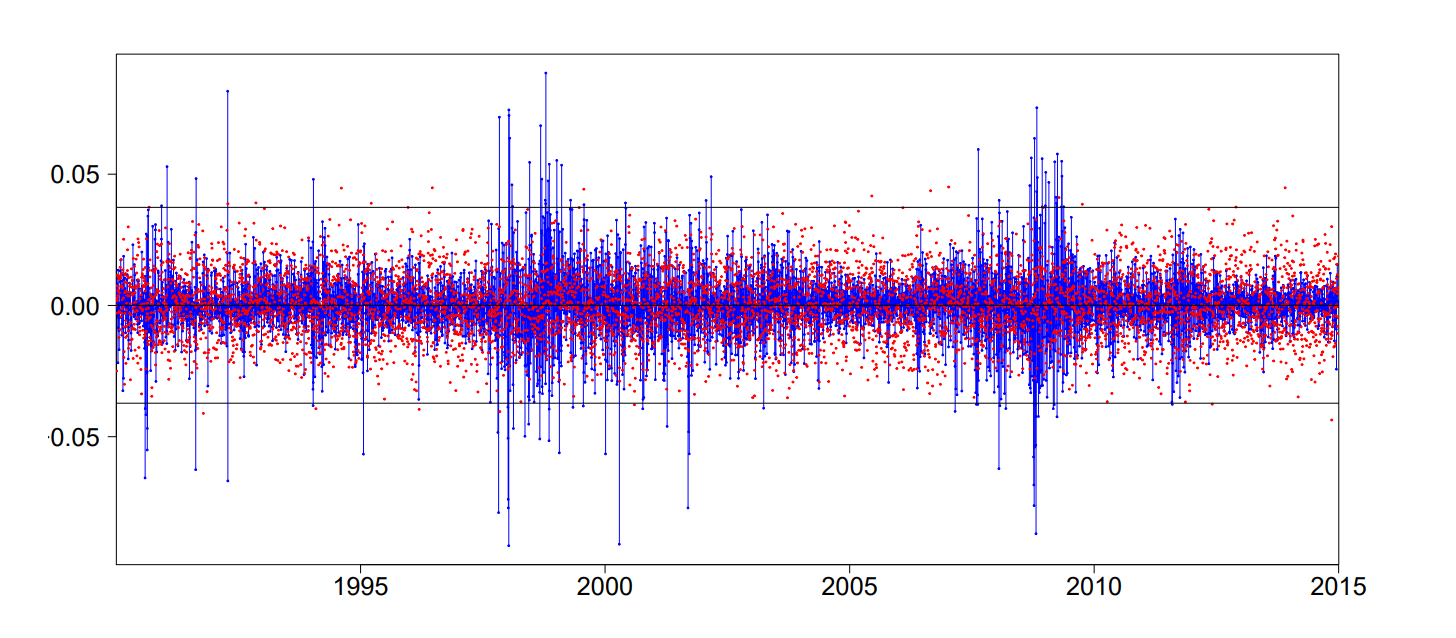
\includegraphics[width=\textwidth]{figures/emprical-vs-gaussian-cdf.png}
    \caption{Market returns (blue) vs normalized Gaussian returns (red) (figure sampled from \cite{book:privault})}
    \label{fig:empirical-vs-gaussian-cdfs}
\end{figure}

\noindent \newline In later section, we will see that in order to alleviate this problem, \textbf{Gram-Charlier expansion} is proposed for higher-order estimate of the empirical CDF of market returns.

\begin{definition}[Cumulants]
    The cumulants of a random variable $X$ is essentially an alternative to moments. The cumulants are derived from the \textbf{cumulant generating function}:
    \begin{align*}
        K_X(t) &= \log M_X(t) = \log \mathbb{E}[e^{tX}] \\
        \kappa_n^X &= K_X^{(n)}(0) \ \ \ (n^{th} \text{ order cumulant})
    \end{align*}
\end{definition}

\textbf{Remark} : We have the following remarks about the cumulant:
\begin{itemize}
    \item $\kappa_1^X=\mathbb{E}[X]$ (Mean).
    \item $\kappa_2^X=Var(X)=\mathbb{E}\Big[ (X - \mu_X)^2 \Big]$ (Variance).
    \item $\kappa_3^X=\mathbb{E}\Big[ (X - \mu_X)^3 \Big]$ (Third central moment).
    \item $\kappa_4^X=\mathbb{E}\Big[ (X - \mu_X)^4 \Big] - 3(\kappa_2^X)^2$.
    \item From the fourth-order cumulant, the cumulant is no longer consistent to central moment.
\end{itemize}

\begin{proposition}{Power-series expansion of $K_X(t)$}{cgf_power_expansion}
    The power-series expansion of the cumulant generating function is defined as followed:
    \begin{align*}
        K_X(t) = \sum_{n=1}^\infty \frac{t^n}{n!}\kappa_n^X
    \end{align*}

    \noindent\newline The above expansion is similar to the following power-series expansion of the moment generating functions:
    \begin{align*}
        M_X(t) = \sum_{n=1}^\infty \frac{t^n}{n!}\mathbb{E}\Big[X^n\Big]
    \end{align*}
\end{proposition}

\begin{definition}[Skewness \& Excess kurtosis]
    The skewness of a random variable $X$ is defined as
    \begin{align*}
        Sk_X = \frac{\kappa_3^X}{(\kappa_2^X)^{3/2}}
    \end{align*}

    The excess kurtosis of a random variable $X$ is defined as
    \begin{align*}
        EK_X = \frac{\kappa_4^X}{(\kappa_2^X)^{4/2}} = \frac{\kappa_4^X}{(\kappa_2^X)^{2}}
    \end{align*}
\end{definition}

\noindent \newline The skewness, intuitively, measures the \textbf{degree of asymmetry} of the probability density function. The excess kurtosis measures the \textbf{peakedness} of the probability density function. An empirical distribution with skewness and excess kurtosis close to zero will be similar to a Gaussian distribution.

\subsection{Gram-Charlier Expansions}
To solve the problem of inaccurate approximation of the probability density function of market returns, Gram-Charlier expansion is proposed for higher order approximation.

\begin{definition}[Hermite polynomial]
    The Hermite polynomial is defined as:
    \begin{align*}
        H_n(x) = (-1)^n \frac{\varphi^{(n)}(x)}{\varphi(x)}
    \end{align*}

    \noindent\newline Where $\varphi(x)$ is the probability density function of the standard normal distribution. The Hermite polynomial is one of the classical orthogonal polynomials used as the orthogonal basis for the Gram-Charlier expansion \cite{article:tanaka} (defined below).
\end{definition}

\begin{definition}[Gram-Charlier Expansion]
    Given a random variable $X$, the probability density function of $X$ can be written as a series expansion as followed:
    \begin{align*}
        f_X(x) &= \sum_{n=0}^\infty \frac{q_n}{\sqrt{\sigma}}H_n(\overline{x})\varphi(\overline{x}) \\
        \text{Where : }&
        \begin{cases}
            q_0 = 1; \ q_1 = q_2 = 0
            \\ \\
            q_n = \frac{1}{n!}\mathbb{E}\Big[H_n(\overline{X}) \Big], \ \ n\ge3
        \end{cases}
    \end{align*}

    \noindent\newline Where $\overline{x}=\frac{x - \kappa_1^X}{\sqrt{\kappa_2^X}} = \frac{x - \mu}{\sigma}$ is the standardized observation and $\overline{X}=\frac{X - \kappa_1^X}{\sqrt{\kappa_2^X}} = \frac{X - \mu}{\sigma}$ is the standardized random variable. $\varphi(.)$ is the PDF of the standard normal distribution.
\end{definition}
\newpage 
\section{Superhedging risk measures}
\subsection{Call and Put options}
\begin{definition}[Put option]
    The \textbf{Put option} provides trader with the right but not the obligation to \textbf{sell} an asset at a strike price $K$ in future time $T$. The payoff of a put option is defined as:
    \begin{align*}
        C = (K - S_T)^+ = \begin{cases}
            K - S_T, & \text{when } K \ge S_T 
            \\ \\
            0, & \text{Otherwise}
        \end{cases} 
    \end{align*}

    \noindent \textit{(The payoff is realized when in the future, the asset price falls below the strike price)}.
\end{definition}


\begin{definition}[Call option]
    The \textbf{Call option} provides trader with the right but not the obligation to \textbf{buy} an asset at a strike price $K$ in future time $T$. The payoff of a call option is defined as:
    \begin{align*}
        C = (S_T - K)^+ = \begin{cases}
            S_T - K, &\text{when } S_T \ge K 
            \\ \\
            0, &\text{Otherwise}
        \end{cases}
    \end{align*}

    \textit{(The payoff is realized when the future price rises above the strike price)}.
\end{definition}

\subsection{Hedging and Pricing options}
\begin{definition}[Cash settlement \& Physical delivery]
    Take put option issuer as the example, there are two modes of issue (deliveries):
    \begin{itemize}
        \item \textbf{Physical delivery} : The option issuer pays the strike price of $K$ to the option holder in exchange for one unit of asset. This usually applies for physical assets like live cattle, fuel, etc.
        \item \textbf{Cash settlement} : The option issuer fulfills the contract by transferring the amount of $(K-S_T)^+$ to the option holder.
    \end{itemize}
\end{definition}

\begin{definition}[Hedging and Pricing options]
    Two issues of options:
    \begin{itemize}
        \item \textbf{Option pricing} : To be fair, option holder have to pay an appropriate price upon signing the contract.
        \item \textbf{Option hedging} : Manage a given portfolio such that it contains the required payoff: $(K-S_T)^+$ for put option and $(S_T-K)^+$ for call option.
    \end{itemize}
\end{definition}

\textbf{Example} : Consider the following example, a risky asset priced at time $t=0$ at $S_0=4$ and taking only two possible values at time $t=1$: $S_1= \{5, 2\}$.

\noindent \newline An option contract promises the payoff:
\begin{align*}
    C = \begin{cases}
        3, \text{if } S_1 = 5
        \\ \\
        0, \text{if } S_1 = 2
    \end{cases}
\end{align*}

\noindent $\bf (ii)$ \textbf{Option hedging} : how to manage the portfolio $(\alpha, \beta)$ such that $\alpha S_1 + \beta$ matches the payoff at $t=1$.

\begin{align*}
    C = \begin{cases}
        3 = 5\alpha + \beta \\ 
        0 = 2\alpha + \beta
    \end{cases} \implies 
    \begin{cases}
        \alpha = 1 \ \text{(Buy stock)} \\ 
        \beta = -2 \ \text{(Borrow from bank)}
    \end{cases}
\end{align*}

\noindent $\bf (i)$ \textbf{Option hedging} : how to charge the option buyer.
\begin{align*}
    V_0 &= \alpha S_0 + \beta \\
        &= 1 \times 4 - 2 = 2 
\end{align*}

\begin{definition}[Arbitrage-free price]
    The \textbf{arbitrage-free price} of an option contract should be the initial cost of creating the portfolio:
    \begin{align*}
        V_0 = \alpha S_0 + \beta
    \end{align*}
\end{definition}

\subsection{Risk-neutral probability \& Market implied probability}
\begin{definition}[Risk-neutral probability]
    With the absence of arbitrage opportunities, the expected payoff ($\mathbb{E}[C]$) should equal the amount of the initial amount $V_0$ invested in the portfolio:
    \begin{align*}
        \mathbb{E}[C] = V_0
    \end{align*}

    \noindent\textbf{Risk-neutral probability} is the probabilities infered from the above equation.
\end{definition}

\begin{definition}[Market-implied probability]
    If we match the theoretical price $\mathbb{E}[C]$ with some market price $M$, we derive the \textbf{Market-implied probability}.
    \begin{align*}
        \mathbb{E}[C] = M
    \end{align*}
\end{definition}

\textbf{Example} : Following the example from the previous section, we have:
\begin{align*}
    \mathbb{E}[C] &= 3 \times P(S_1 = 5) + 0 \times P(S_1 = 2) \\
        &= 3 \times P(S_1 = 5)
\end{align*}

\noindent Equating the above expected payoff to the initial value invested in the option, we have:
\begin{align*}
    \mathbb{E}[C] = V_0 \implies 3\times P(S_1 = 5) = 2 \implies 
    \begin{cases}
        P(S_1 = 5) &= \frac{2}{3} 
        \\ \\
        P(S_1 = 2) &= \frac{1}{3}
    \end{cases}
\end{align*}

\noindent On the other hand, the market-implied probability is:
\begin{align*}
    \begin{cases}
        P(S_1 = 5) &= \frac{M}{3} 
        \\ \\
        P(S_1 = 2) &= \frac{3 - M}{3}
    \end{cases}
\end{align*}

\newpage 
\section{Value at Risk (VaR)}

\subsection{Risk Measures}
\begin{definition}[Risk measure]
    A \textbf{risk measure} is a mapping that assigns a value $V_X$ to a given \textbf{payoff} random variable $X$.
\end{definition}

\noindent\newline These are a few examples of risk measures:
\begin{itemize}
    \item The \textbf{expected value premium principle} : 
    \begin{align*}
        V_X=\mathbb{E}[X] + \alpha\mathbb{E}[X]
    \end{align*}
    \noindent For some $\alpha\ge0$. For $\alpha=0$, $V_X=\mathbb{E}[X]$ is called the \textbf{pure premium risk measure}.

    \item The \textbf{standard deviation premium principle} : 
    \begin{align*}
        V_X = \mathbb{E}[X] - \alpha\sqrt{Var(X)}
    \end{align*}
    \noindent For some $\alpha\ge0$.

    \item The \textbf{Conditional Tail Expectation (CTE)} over negative payoff $X$ is defined as followed:
    \begin{align*}
        CTE_X = \mathbb{E}\Big[ X|X<0 \Big] = \frac{\mathbb{E}[X\1{X<0}]}{P(X<0)}
    \end{align*}
\end{itemize}

\begin{definition}[Coherent risk measure]
    A risk measure $V$ is said to be \textbf{coherent} if it satisfies the following properties:
    \begin{itemize}
        \item \textbf{Monotonicity : } $X \le Y\implies V_X \le V_Y$.
        \item \textbf{Positive Homogeneity : } $V_{\lambda X} = \lambda V_X, \lambda > 0$.
        \item \textbf{Translation invariance : } $V_{\mu + X} = \mu + V_X$.
        \item \textbf{Sub-additivity : } $V_{X+Y} \le V_X + V_Y$.
    \end{itemize}
\end{definition}

\begin{definition}[Distortion risk measure]
    A \textbf{distortion risk measure} is any risk measure of the form:
    \begin{align*}
        M_X = \mathbb{E}\Big[ Xg_X(X) \Big]
    \end{align*}

    \noindent Where $g_X$ is \textbf{non-negative, non-decreasing} function satisfying:
    \begin{itemize}
        \item $\mathbb{E}\Big[ g_X(X) \Big] = 1$.
        \item \textbf{Positive homogeneity : } $g_{\lambda X}(\lambda x) = g_X(x), \ \lambda > 0$.
        \item \textbf{Translation invariance : } $g_{X + \mu}(x+\mu) = g_X(x)$.
    \end{itemize}

    \noindent\newline The distortion risk measure $M_X$ satisfies the following properties:
    \begin{itemize}
        \item \textbf{Positive homogeneity : } For $\lambda > 0$, we have
        \begin{align*}
            \mathbb{E}\Big[ \lambda X g_{\lambda X}(\lambda X)\Big] = \mathbb{E}\Big[ \lambda X g_{X}(X)\Big] = \lambda \mathbb{E}\Big[ Xg_X(X) \Big]
        \end{align*}

        \item \textbf{Translation invariance : } For $\mu \ge 0$, we have
        \begin{align*}
            \mathbb{E}\Big[ (X + \mu)g_{X+\mu}(X+\mu) \Big] = \mathbb{E}\Big[ (X + \mu)g_{X}(X) \Big] = \mathbb{E}\Big[ Xg_X(X) \Big] + \mu\mathbb{E}\Big[ g_{X}(X) \Big] = \mathbb{E}\Big[ Xg_X(X) \Big] + \mu
        \end{align*}
    \end{itemize}
\end{definition}

\subsection{Quantile Risk Measures}
\subsubsection{Cumulative Distribution Function}
\begin{definition}[Cumulative Distribution Function (CDF)]
    The CDF of a random variable $X$ is defined as a function $F_X:\mathbb{R} \to [0,1]$ defined by:
    \begin{align*}
        F_X(x) = P(X \le x), \ \ x \ge 0
    \end{align*}
    \noindent Any CDF satisfies the following properties:
    \begin{itemize}
        \item \textbf{Non-decreasing}.
        \item \textbf{Right-continuous}.
        \item \textbf{$\lim_{x\to\infty F_X(x) = 1}$}.
        \item \textbf{$\lim_{x\to-\infty F_X(x) = 0}$}.
    \end{itemize}
\end{definition}

\noindent (The following are fundamental results of the CDFs, the proof will not be provided).
\begin{proposition}{Continuity of CDFs}{cont_of_cdf}
    For any non-decreasing sequence $(x_n)_{n\ge 1}$ such that $x_n \to x\in\mathbb{R}$, we have:
    \begin{align*}
        \lim_{n\to\infty}F_X(x_n) = \lim_{n\to\infty} P(X \le x_n) = P(X < x)
    \end{align*}
\end{proposition}

\begin{proposition}{Discontinuity of CDFs}{discont_of_cdf}
    The CDF of a random variable $X$ is right-continuous (not both way continuous). Hence, when there is a case where the CDF is discontinuous (figure \ref{fig:cdf-with-discont}) at a given point $x\in\mathbb{R}$, we can compute the probability that $X=x$:
    \begin{align*}
        P(X=x) = P(X\le x) - P(X < x) = F_X(x) - \lim_{y\to x^-}F_X(y)
    \end{align*}
\end{proposition}

\begin{figure}[ht]
    \centering
    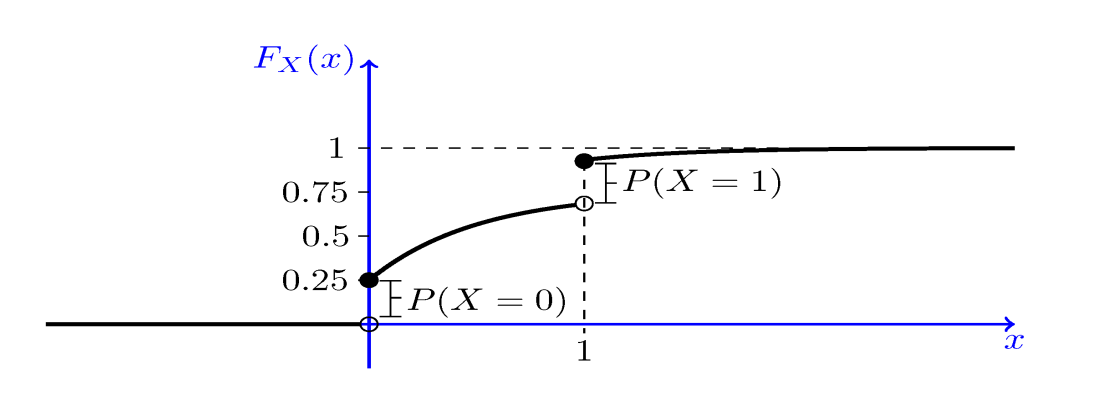
\includegraphics[width=\textwidth]{figures/cdf_with_discont.png}
    \caption{CDF with discontinuity (figure sampled from \cite{book:privault})}
    \label{fig:cdf-with-discont}
\end{figure}

\begin{definition}[Quantile]
    Given a random variable $X$ with the CDF $F_X:\mathbb{R}\to[0,1]$ and a level $p\in(0,1)$. The $p$-quantile of $X$ is given by:
    \begin{align*}
        q_X^p = \inf\Big\{x\in\mathbb{R} : F_X(x) \ge p\Big\}
    \end{align*}
\end{definition}

\noindent\newline \textbf{Remark} : Note that by proposition \ref{prop:discont_of_cdf}, we have:
    $P(X = q_X^p) = F_X(q_X^p) - \lim_{y \to (q_X^p)^-}F_X(y)$. Hence, when there is no discontinuity in $q_X^p$ ($P(X = q_X^p)=0$), we have :
\begin{align*}
    \boxed{
    P(X= q_X^p)=0 \implies p = \lim_{y \to (q_X^p)^-}F_X(y) = F_X(q_X^p)    
    }
\end{align*}

\subsubsection{Empirial Cumulative Distribution Function}
\begin{definition}[Empirical Cumulative Distribution Function (E-CDF)]
    The \textbf{Empirical Cumulative Distribution Function (E-CDF)} of an $N$-point dataset $\{x_1, \dots, x_N\}$ is estimated as:
    \begin{align*}
        F_N(x) = \frac{1}{N}\sum_{n=1}^N \1{x_n \le x}, \ \ x\ge0
    \end{align*}
\end{definition}

\subsection{Value at Risk (VaR)}
\begin{definition}[Value at Risk (VaR)]
    The \textbf{Value at Risk (VaR)} of a random variable $X$ at level $p\in(0,1)$ is the $p$-quantile of $X$:
    \begin{align*}
        \boxed{
            V_X^p = q_X^p = \inf\Big\{
                x \in \mathbb{R} : F_X(x) \ge p
            \Big\}
        }
    \end{align*}
\end{definition}

\begin{proposition}{Properties of Value at Risk}{properties_of_var}
    The Value at Risk (VaR) has the following properties:
    \begin{itemize}
        \item $(i)$ The function $p\to V_X^p$ is \textbf{non-decreasing, left-continuous} and it \textbf{admits limit from the right}.
        \item $(ii) \ V_X^p \le x \iff p\le P(X\le x)$.
        \item $(iii) \ V_{-X}^p = -V_X^{1-p}$.
    \end{itemize}
\end{proposition}

\begin{proof*}[Proposition \ref{prop:properties_of_var}]
    Proving each property, we have:
    \begin{subproof}{\newline Claim : $p\to V_X^p$ is non-decreasing, left-continuous and admits limit from the right}
        The function $p\to V_X^p$ (called the quantile function) is the \textbf{generalized inverse} of the Cumulative Distribution Function.

        \noindent\newline By proposition 2.3 - \cite{article:Embrechts2013}, since $F_X(x)$ is non-decreasing, the generalized inverse of it is non-decreasing, left-continuous and admits limits on the right.
    \end{subproof}

    \begin{subproof}{\newline Claim : $V_X^p \le x \iff p\le P(X\le x)$}
        Trivial due to the definition of Value at Risk (VaR).
    \end{subproof}

    \begin{subproof}{\newline Claim : $V_{-X}^p = -V_X^{1-p}$}
        We have:
        \begin{align*}
            F_{-X}(x) &= P(-X \le x) = P(X \ge -x) \\
                &= 1 - P(X < -x) = 1 - P(X \le -x) \\
                &= 1 - F_X(-x)
        \end{align*}

        \noindent Hence, we have:
        \begin{align*}
            p = F_{-X}(F_{-X}^{-1}(p)) = 1 - F_X(-F_{-X}^{-1}(p))
        \end{align*}
        \noindent Which yields:
        \begin{align}
            V_{-X}^p = F_{-X}^{-1}(p) = -F_{-X}^{-1}(1-p) = -V_X^{1-p}
        \end{align}
    \end{subproof}
\end{proof*}

\begin{theorem}{Coherence of Value at Risk (VaR)}{coherence_of_var}
    Value at Risk (VaR) satisfies:
    \begin{itemize}
        \item $(i)$ Monotonicity.
        \item $(ii)$ Positive homogeneity and translation invariance.
        \item $(iii)$ \textbf{But NOT} sub-additivity.
    \end{itemize}
\end{theorem}

\begin{proof*}[Theorem \ref{thm:coherence_of_var}]
    
\end{proof*}
    

\begin{definition}[Gaussian Value at Risk (G-VaR)]
    Given $X\sim \mathcal{N}(\mu_X, \sigma_X^2)$, we have:
    \begin{align*}
        \boxed{
            V_X^p = \mu_X + \sigma_X q_Z^p
        }
    \end{align*}
    \noindent Where the normal quantile $q_Z^p = V_Z^p$ at level $p$ satisfies:
    \begin{align*}
        \Phi(q_Z^p) = P(Z \le q_Z^p) = p, \ \ Z \sim \mathcal{N}(0,1)
    \end{align*}
    \noindent Meaning, we have:
    \begin{align*}
        V_X^p = \mu_X + \sigma_X \Phi^{-1}(p)
    \end{align*}
\end{definition}

\begin{lemma}{$X=V_X^U, P(U \ge p) \ne P(V_X^U \ge V_X^p)$}{x_equal_vx_power_u}
    We can write any random variable $X$ as:
    \begin{align*}
        X = V_X^U, \ U \sim Uniform(0,1)
    \end{align*}

    \noindent However, for any $p\in(0,1)$, we do not always have $P(U \ge p) = P(V_X^U \ge V_X^p)$. Instead, we have the following relationship:
    \begin{align*}
        P(V_X^U \ge V_X^p) &= P((V_X^U \ge V_X^p) \cap (U \ge p)) + P((V_X^U \ge V_X^p) \cap (U < p)) \\
        \text{Or : } P(X \ge V_X^p) &= P((X \ge V_X^p) \cap (U \ge p)) + P((X \ge V_X^p) \cap (U < p))
    \end{align*}

    \noindent This implies that the event $(V_X^U \ge V_X^p) \cap (U < p)$ can indeed have non-zero probability measure and it happens when there are discontinuities.
\end{lemma}

\begin{proof*}[Lemma \ref{lem:x_equal_vx_power_u}]
    By proposition \ref{prop:properties_of_var}, we have $P(V_X^p\le x) \iff p \le P(X\le x)$. Hence:
    \begin{align*}
        P(V_X^U \le x) &= P(U \le P(X\le x)) = P(X\le x) = F_X(x)
    \end{align*}
    \noindent To prove the second point, we have the following visual representation in figure \ref{fig:lemma3.1_illustration}.
    \begin{figure}[ht]
        \centering
        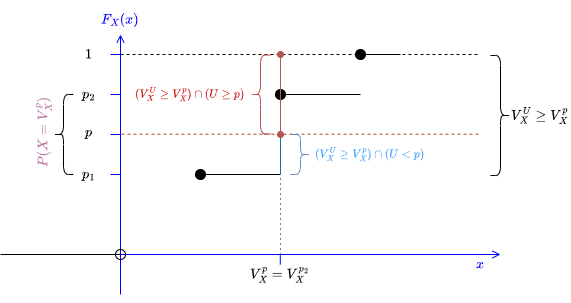
\includegraphics[width=\textwidth]{figures/lemma3.1-illustration.png}
        \caption{$P(V_X^U \ge V_X^p) = P((V_X^U \ge V_X^p) \cap (U \ge p)) + P((V_X^U \ge V_X^p) \cap (U < p))$}
        \label{fig:lemma3.1_illustration}
    \end{figure}
\end{proof*}

\begin{proposition}{Discontinuity at $V_X^p$}{discont_at_var}
    Let $V_X^p$ be the Value at Risk of a random variable $X$ at level $p\in(0,1)$. Then, we have:
    \begin{align*}
        P(X = V_X^p) = 0 \iff p = F_X(V_X^p) = \lim_{y\to x^-}F_X(y)
    \end{align*}

    \noindent\newline In other words, if there is no discontinuity at $V_X^p$, then $p = F_X(V_X^p)$.
\end{proposition}

\begin{proof*}[Proposition \ref{prop:discont_at_var}]
    By proposition \ref{prop:discont_of_cdf}, we have that when $P(X=V_X^p)=0$, we have $F_X(V_X^p) = P(X < V_X^p) = \lim_{y\to x^- F_X(y)}$. Now, we have to prove that $p=F_X(V_X^p)$. 

    \noindent\newline We have:
    \begin{align*}
        F_X(V_X^p) &= P(X \le V_X^p) = 1 - P(X > V_X^p) \\
        &= 1 - P(X \ge V_X^p) = 1 - P(V_X^U \ge V_X^p) \\
        &= 1 - P(U \ge p) \\
        &= 1 - (1 - p) = p
    \end{align*}

    \noindent\newline \textbf{Remark} : Note that by the visual representation in figure \ref{fig:lemma3.1_illustration}, when $P(X=V_X^p)=0$, we have:
    \begin{align*}
        P(V_X^U \ge V_X^p) = P(V_X^U \ge V_X^p \cap (U \ge p)) = P(U\ge p) 
    \end{align*}
\end{proof*}

\newpage
\section{Expected Shortfall}
\subsection{Tail Value at Risk (TVaR)}
\textbf{Overview} : One common shortcoming of Value at Risk is the inability to capture the behavior of the distribution beyond $V_X^p$ (as illustrated in figure \ref{fig:var-shortcoming}). Hence, one way to remedy this shortcoming is to taking the average of Value at Risk beyond the level $p$.
\begin{figure}[ht]
    \centering
    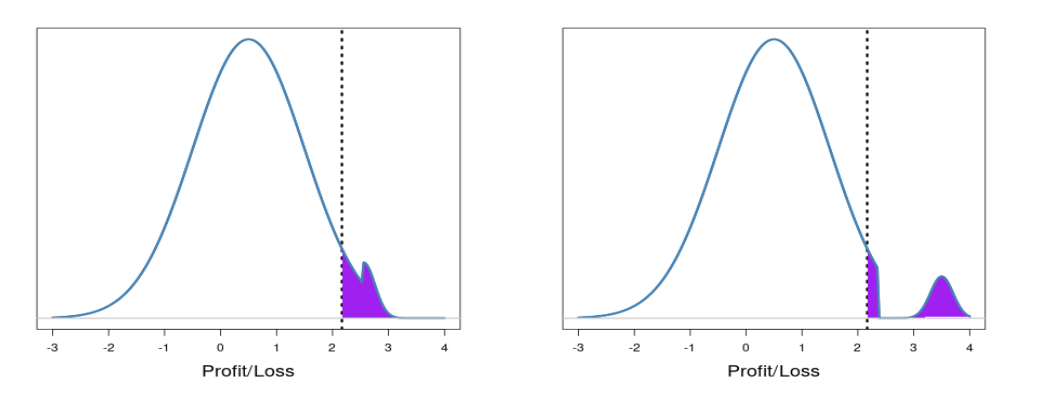
\includegraphics[width=\textwidth]{figures/var_shortcoming.png}
    \caption{Two distributions having the same $V_X^{0.95} = 2.145$ (figure sampled from \cite{book:privault})}
    \label{fig:var-shortcoming}
\end{figure}

\begin{definition}[Tail Value at Risk (TVaR)]
    The Tail Value at Risk (TVaR) of a random variable $X$ at the level $p\in(0,1)$ is defined by the following average:
    \begin{align*}
        \boxed{
            TV_X^p = \frac{1}{1-p} \int_p^1 V_X^qdq
        }
    \end{align*}

    \noindent Note that $p \to V_X^p$ is a non-decreasing function (Proposition \ref{prop:properties_of_var}). Therefore, we always have:
    \begin{align*}
        TV_X^p = \frac{1}{1-p}\int_p^1 V_X^{\bf q}dq \ge \frac{1}{1-p}\int_p^1 V_X^{\bf p}dq = V_X^p
    \end{align*}
\end{definition}

\subsection{Conditional Tail Expectation (CTE)}
\textbf{Overview} : Conditional Tail Expectation is another measure that takes into account "what happens beyond $V_X^p$. However, instead of taking the uniform average as Tail Value at Risk, Conditional Tail Expectation takes the conditional expectation of $X$ conditioned on the event that $X > V_X^p$.

\begin{definition}[Conditional Expectation]
    Given a random variable $X$ and an event $A$ such that $P(A)>0$. The conditional expectation of $X$ given the event $A$ is defined as:
    \begin{align*}
        \mathbb{E}[X|A] = \frac{1}{P(A)}\mathbb{E}[X\1{A}]
    \end{align*}
\end{definition}

\begin{definition}[Conditional Tail Expectation (CTE)]
    Given a random variable $X$ such that $P(X>V_X^p)>0$ at a level $p\in (0,1)$. The \textbf{Conditional Tail Expectation} of $X$ at level $p$ is defined as:
    \begin{align*}
        \boxed{
            CTE_X^p = \mathbb{E}\Big[
                X \Big| X > V_X^p
            \Big] = \frac{\mathbb{E}[X\1{X>V_X^p}]}{P(X>V_X^p)}
        }
    \end{align*}

    \noindent The Conditional Tail Expectation can be written as a Distortion Risk Measure $CTE_X^p=\mathbb{E}\Big[ Xf_X(X)\Big]$ with the distortion function:
    \begin{align*}
        \boxed{
            f_X(x) = \frac{1}{P(X>V_X^p)}\1{x>V_X^p}
        }
    \end{align*}
\end{definition}

\begin{proposition}{$CTE_X^p - V_X^p$}{cte_and_var_diff}
    For any $p\in(0,1]$, we have $CTE_X^p > \mathbb{E}[X]$ and $CTE_X^p > V_X^p$. Specifically:
    \begin{align*}
        CTE_X^p = \mathbb{E}\Big[ X\Big|X>V_X^p \Big] = V_X^p + \mathbb{E}\Big[(X-V_X^p)^+ | X > V_X^p\Big]
    \end{align*}
\end{proposition}

\begin{proof*}[Proposition \ref{prop:cte_and_var_diff}]
    We have :
    \begin{align*}
        \mathbb{E}\Big[ X | X > V_X^p \Big] 
            &= \frac{1}{P(X>V_X^p)}\mathbb{E}\Big[ X\1{X > V_X^p} \Big] \\
            &= \frac{1}{P(X>V_X^p)}\Bigg[ \mathbb{E}\Big[ (X - V_X^p) \1{X > V_X^p} \Big] + V_X^p\mathbb{E}\Big[ \1{X > V_X^p} \Big] \Bigg] \\
            &= \frac{1}{P(X>V_X^p)}\Bigg[ \mathbb{E}\Big[ (X - V_X^p) \1{X > V_X^p} \Big] + V_X^pP(X>V_X^p) \\
            &= V_X^p + \frac{1}{P(X>V_X^p)} \mathbb{E}\Big[ (X - V_X^p) \1{X > V_X^p} \Big] \\
            &= V_X^p + \mathbb{E}\Big[ X - V_X^p | X > V_X^p \Big]
    \end{align*}
\end{proof*}

\begin{proposition}{When $CTE_X^p=TV_X^p$}{when_cte_equal_tvar}
    When $P(X=V_X^p)=0$, meaning there is no discontinuity at $V_X^p$, then we have:
    \begin{align*}
        P(X=V_X^p)=0 \iff CTE_X^p = TV_X^p
    \end{align*}
\end{proposition}

\begin{proof*}[Proposition \ref{prop:when_cte_equal_tvar}]
    By figure \ref{fig:lemma3.1_illustration}, we can see that when $P(X=V_X^p)=0$, we have, with probability one, $P(V_X^U > V_X^p) = P(V_X^U \ge V_X^p) = P(U \ge p)$. Hence:
    \begin{align*}
        CTE_X^p &= \mathbb{E}\Big[ X | X > V_X^p\Big] \\
        &= \frac{1}{P(X>V_X^p)}\mathbb{E}\Big[ X\1{X > V_X^p} \Big] \\
        &= \frac{1}{P(U \ge p)}\mathbb{E}\Big[ X\1{U \ge p} \Big] \\
        &= \frac{1}{P(U \ge p)}\mathbb{E}\Big[ V_X^U\1{U \ge p} \Big] \\
        &= \frac{1}{1-p} \int_p^1 V_X^qdp = TV_X^p
    \end{align*}
\end{proof*}

\begin{definition}[Gaussian CTE (G-CTE)]
    Given $X\sim \mathcal{N}(\mu_X, \sigma_X^2)$, we have:
    \begin{align*}
        \boxed{
        CTE_X^p = \mu_X + \frac{\sigma_X}{1-p}\varphi(V_Z^p) = \mu_X + \frac{\sigma_X}{(1-p)\sqrt{2\pi}}\exp\Bigg( -\frac{(V_Z^p)^2}{2} \Bigg)
        }
    \end{align*}
    \noindent Or we can write:
    \begin{align*}
        CTE_X^p = \mu_X + \frac{\sigma_X}{(1-p)\sqrt{2\pi}}\exp\Bigg( -\frac{(q_Z^p)^2}{2} \Bigg)
    \end{align*}

    \noindent $\varphi(.)$ is the standard normal probability density function.
\end{definition}

\subsection{Expected Shortfall (ES)}
\begin{definition}[Expected Shortfall (ES)]
    Given a random variable $X$, the \textbf{Expected Shortfall (ES)} at the level $p \in (0,1)$ is defined by
    \begin{align*}
        \boxed{
            ES_X^p = V_X^p + \frac{1}{1-p} \mathbb{E}\Big[ 
                (X - V_X^p)\1{X\ge V_X^p}
            \Big]
        }
    \end{align*}

    \noindent The Expected Shortfall (ES) can be written as a Distortion Risk Measure $ES_X^p=\mathbb{E}\Big[ Xf_X(X) \Big]$ defined as:
    \begin{align*}
        \boxed{
            f_X(x) = \frac{1}{1-p}\Bigg( 
                \1{X > V_X^p} + \1{P(X=V_X^p) > 0}\1{X=V_X^p}\frac{1-p-P(X>V_X^p)}{P(X=V_X^p)}
            \Bigg)
        }   
    \end{align*}
    \noindent\newline This can be deduced from proposition \ref{prop:alternative_dfn_es} below.
\end{definition}

\begin{proposition}{Altenative definition of $ES_X^p$}{alternative_dfn_es}
    The Expected Shortfall (ES) at level $p\in(0,1)$ can be written as:
    \begin{align*}
        ES_X^p = \frac{1}{1-p}\mathbb{E}[X\1{X\ge V_X^p}] + \frac{V_X^p}{1-p}\Big(1-p-P(X\ge V_X^p)\Big)
    \end{align*}
\end{proposition}

\begin{proof*}[Proposition \ref{prop:alternative_dfn_es}]
    We have:
    \begin{align*}
        ES_X^p 
            &= V_X^p + \frac{1}{1-p}\mathbb{E}\Big[ (X - V_X^p)\1{X\ge V_X^p} \Big] \\
            &= V_X^p + \frac{1}{1-p}\mathbb{E}\Big[X-V_X^p \Big| X\ge V_X^p \Big] P(X\ge V_X^p) \\
            &= V_X^p + \frac{P(X\ge V_X^p)}{1-p}\Bigg\{ \mathbb{E}\Big[ X| X \ge V_X^p \Big] - V_X^p \Bigg\} \\
            &= V_X^p + \frac{P(X\ge V_X^p)}{1-p}\Bigg\{ \frac{1}{P(X\ge V_X^p)} \mathbb{E}\Big[ X\1{X\ge V_X^p} \Big] - V_X^p \Bigg\} \\
            &= \frac{1}{1-p}\mathbb{E}\Big[ X\1{X\ge V_X^p} \Big] + V_X^p \Big( 1 - \frac{P(X\ge V_X^p)}{1-p} \Big) \\
            &= \frac{1}{1-p}\mathbb{E}\Big[ X\1{X\ge V_X^p} \Big] + \frac{V_X^p}{1-p}\Big( 1 - p - P(X\ge V_X^p) \Big)
    \end{align*}
\end{proof*}

\begin{corollary}{$ES_X^p$ when $P(X=V_X^p) = 0$}{es_when_continuous}
    As a direct consequence of Proposition \ref{prop:alternative_dfn_es}, we have:
    \begin{align*}
        P(X=V_X^p) = 0 \iff ES_X^p = CTE_X^p
    \end{align*}

    \noindent By proposition \ref{prop:when_cte_equal_tvar}, we can even have:
    \begin{align*}
        P(X=V_X^p) = 0 \iff ES_X^p = CTE_X^p = TV_X^p
    \end{align*}
\end{corollary}

\begin{proof*}[Corollary \ref{coro:es_when_continuous}]
    When $P(X=V_X^p) = 0$, we have $p=F_X(V_X^p)=P(X\le V_X^p)=P(X<V_X^p)$. Hence, by the definition of expected shortfall, we have:
    \begin{align*}
        ES_X^p 
        &= V_X^p + \frac{1}{1-p}\mathbb{E}\Big[ (X - V_X^p)\1{X\ge V_X^p} \Big] \\
        &= V_X^p + \frac{1}{1 - P(X \le V_X^p)}\mathbb{E}\Big[ (X - V_X^p)\1{X\ge V_X^p} \Big] \\
        &= V_X^p + \frac{1}{P(X > V_X^p)}\mathbb{E}\Big[ (X - V_X^p)\1{X\ge V_X^p} \Big] \\
        &= V_X^p + \frac{1}{P(X > V_X^p)}\mathbb{E}\Big[ X - V_X^p \Big| X \ge V_X^p \Big] P(X\ge V_X^p) \\
        &= V_X^p + \frac{1}{P(X > V_X^p)}\mathbb{E}\Big[ X - V_X^p \Big| X > V_X^p \Big] P(X > V_X^p) \\
        &= V_X^p + \mathbb{E}\Big[ X - V_X^p \Big| X > V_X^p \Big] \\
        &= \mathbb{E}\Big[ X \Big| X > V_X^p \Big] = CTE_X^p
    \end{align*}
\end{proof*}

\begin{proposition}{$ES_X^p$ and $TV_X^p$ for any $p\in(0,1)$}{es_tv_any_p}
    This proposition proves a much stronger result than Corollary \ref{coro:es_when_continuous}. For any $p\in(0,1)$ (not just when $P(X = V_X^p) = 0$), we have:
    \begin{align*}
        ES_X^p = TV_X^p = \frac{1}{1-p}\int_p^1 V_X^qdq
    \end{align*}
\end{proposition}

\begin{proof*}[Proposition \ref{prop:es_tv_any_p}]
    We first prove the following claim:

    \begin{subproof}{\newline Claim 1 : $V_X^p\Big(1-p-P(X\ge V_X^p) \Big)=-\mathbb{E}\Big[ X\1{ ( X\ge V_X^p ) \cap (U<p)} \Big]$}
        For $U\sim Uniform(0,1)$, note that:
        \begin{align*}
            P(U \ge p) &= 1 - p = \mathbb{E}\Big[ \1{U \ge p} \Big] \\
            P(X \ge V_X^p) &= \mathbb{E}\Big[ \1{X \ge V_X^p} \Big]
        \end{align*}

        \noindent (Note that it is tempting to conclude that $P(X\ge V_X^p)=P(V_X^U \ge V_X^p) = P(U\ge p)$. However, this is not true by lemma \ref{lem:x_equal_vx_power_u} because we can have $V_X^{p_1}\ge V_X^{p_2}$ for $p_1<p_2$ if there is discontinuity between $p_1$ and $p_2$). 

        \noindent \newline Now, we have:
        \begin{align*}
            V_X^p\Big( 1 - p - P(X\ge V_X^p) \Big) 
                &= V_X^p\Bigg( 
                    \mathbb{E}\Big[ \1{U\ge p} \Big] - \mathbb{E}\Big[ \1{X \ge V_X^p} \Big]
                \Bigg) \\
                &= - V_X^p \mathbb{E}\Big[ \1{X \ge V_X^p} - \1{U\ge p} \Big] \\ 
                &= - V_X^p \mathbb{E}\Big[ \1{(X \ge V_X^p)\setminus (U \ge p)} \Big] \\ 
                &= - V_X^p \mathbb{E}\Big[ \1{(X \ge V_X^p)\cap (U < p)} \Big] \\ 
        \end{align*}

        \noindent \newline As illustrated in figure \ref{fig:lemma3.1_illustration}, when the event $(V_X^U \ge V_X^p)\cap (U<p)$ occurs, we have $X=V_X^p$. Hence, we can also write:
        \begin{align*}
            V_X^p\Big( 1 - p - P(X\ge V_X^p) \Big) 
                &= - V_X^p \mathbb{E}\Big[ \1{(X \ge V_X^p)\cap (U < p)} \Big] \\ 
                &= - \mathbb{E}\Big[ X \1{(X \ge V_X^p)\cap (U < p)} \Big]
        \end{align*}
    \end{subproof}

    \begin{subproof}{\newline Claim 2 : $ES_X^p = TV_X^p$}
        From the above, we have:
        \begin{align*}
            ES_X^p &= \frac{1}{1-p}\mathbb{E}\Big[ X\1{X\ge V_X^p}\Big] + \frac{V_X^p}{1-p}\Big( 1 - p - P(X\ge V_X^p) \Big) \ \ \ \text{(By proposition \ref{prop:alternative_dfn_es})} \\
            &= \frac{1}{1-p}\Bigg( \mathbb{E}\Big[ X\1{X\ge V_X^p}\Big] - \mathbb{E}\Big[ X \1{(X \ge V_X^p)\cap (U < p)} \Big] \Bigg) \\
            &= \frac{1}{1-p}\mathbb{E}\Big[ X\1{(X\ge V_X^p) \cap (X\ge V_X^p)^c \cup (U \ge p)}\Big] \\
            &= \frac{1}{1-p}\mathbb{E}\Big[ X\1{U \ge p}\Big] \\
            &= \frac{1}{1-p}\mathbb{E}\Big[ V_X^U\1{U \ge p}\Big] \\
            &= \frac{1}{1-p}\int_p^1 V_X^qdq = TV_X^p
        \end{align*}
    \end{subproof}
\end{proof*}

\begin{theorem}{Coherence of $ES_X^p$ and $TV_X^p$}{coherence_es_tv}
    \textbf{Expected shortfall (ES)} and \textbf{Tail Value at Risk (TVaR)} are coherent risk measures. The \textbf{Conditional Tail Expectation (CTE)} is generally not coherent (incoherent when $P(X=V_X^p)>0$). 
\end{theorem}

\begin{proof*}[Theorem \ref{thm:coherence_es_tv}]
    Since Expected Shortfall (ES) and Tail Value at Risk (TVaR) are the same for any $p\in(0,1)$, we can use either measure to prove coherence. In this proof, we will use Tail Value at Risk (TVaR).

    \begin{subproof}{\newline (i) Monotonicity}
        Let $X, Y$ be random variables such that $X \le Y$. We have:
        \begin{align*}
            TV_X^p = \frac{1}{1-p}\int_p^1 V_X^qdq \le \frac{1}{1-p}\int_p^1 V_Y^qdq = TV_Y^p \ \ \text{(Since VaR is monotone)}
        \end{align*}
    \end{subproof}
    
    \begin{subproof}{\newline (ii) Positive homogeneity and translation invariance}
        Let $\lambda > 0$ and $\mu \ge 0$, we have:
        \begin{align*}
            TV_{\mu + \lambda X}^p &= \frac{1}{1-p}\int_p^1 V_{\mu + \lambda X}^q dq \\
            &= \int_p^1 \Big( \mu + \lambda V_X^q \Big)dq \\
            &= \mu + \frac{\lambda}{1-p}\int_p^1 V_X^qdq \\
            &= \mu + \lambda TV_X^p
        \end{align*}
    \end{subproof}

    \begin{subproof}{\newline (iii) Sub-additivity}
        Since the Expected Shortfall (ES) can be written as a Distortion Risk Measure with the following distortion function:
        \begin{align*}
            f_X(x) = \frac{1}{1-p}\Bigg( 
                \1{X > V_X^p} + \1{P(X=V_X^p) > 0}\1{X=V_X^p}\frac{1-p-P(X>V_X^p)}{P(X=V_X^p)}
            \Bigg)
        \end{align*}

        \noindent\newline We have:
        \begin{align*}
            (1 - p)(ES_{X+Y}^p - ES_X^p - ES_Y^p) 
                &= (1 - p)\Bigg( \mathbb{E}\Big[ (X+Y)f_{X+Y}(X + Y)\Big] - \mathbb{E}\Big[ Xf_X(X) \Big] - \mathbb{E}\Big[ Yf_Y(Y) \Big] \Bigg) \\
                &= (1 - p)\Bigg( \mathbb{E}\Big[ X\Big(f_{X+Y}(X+Y) - f_X(X)\Big) \Big] + \mathbb{E}\Big[ Y\Big(f_{X+Y}(X+Y) - f_Y(Y)\Big)\Big] \Bigg) \\
                &\le V_X^p \mathbb{E}\Big[ f_{X+Y}(X+Y) - f_X(X)\Big] + V_Y^p \mathbb{E}\Big[ f_{X+Y}(X+Y) - f_Y(Y) \Big] \\
                &= V_X^p(1 - 1) + V_Y^p(1-1) = 0 \\
                \implies ES_{X+Y}^p &\le ES_X^p + ES_Y^p
        \end{align*}
    \end{subproof}
\end{proof*}

\subsection{Conclusion (Asset risk measures)}
\textbf{Remark} : As a concluding remark, we have the following
\begin{align*}
    \text{When } P(X = V_X^p) 
    \begin{cases}
        = 0   &\implies TV_X^p = ES_X^p    = CTE_X^p \\ \\
        \ne 0 &\implies TV_X^p = ES_X^p \ne CTE_X^p
    \end{cases}
\end{align*}

\noindent\newline \textbf{Summary of asset risk measures} :
\begin{table}[ht]
\begin{center}
\resizebox{\textwidth}{!}{
\begin{tabular}{l | r | r | r }
\toprule
\textbf{Risk measure} & \textbf{Definition} & \textbf{Gaussian} & \textbf{Others} \\
    \midrule\midrule
    \textbf{VaR ($V_X^p$)}          
        & $\inf\Big\{ x \in \mathbb{R} : P(X\le x) \ge p \Big\}$                    
        & $\mu_X + \sigma_Xq_Z^p$    
        & N/A
        \\
    \midrule

    \textbf{TVaR ($TV_X^p$)}         
        & $\frac{1}{1-p}\int_p^1 V_X^qdq$                    
        & N/A     
        & N/A
        \\
    \midrule
    
    \textbf{ES ($ES_X^p$)}           
        & $V_X^p + \frac{1}{1-p}\mathbb{E}\Big[ (X-V_X^p)\1{X\ge V_X^p} \Big]$                    
        & N/A        
        & $\frac{1}{1-p}\Big( \mathbb{E}[X\1{X\ge V_X^p}] + V_X^p(1-p-P(X\ge V_X^p)) \Big)$
        \\
    \midrule
    
    \textbf{CTE ($CTE_X^p$)}          
        & $\mathbb{E}\Big[ X \Big| X > V_X^p \Big]$                   
        & $\mu_X + \frac{\sigma_X}{1-p}\varphi(q_Z^p)$ 
        & $V_X^p + \mathbb{E}\Big[ X - V_X^p | X > V_X^p \Big]$
        \\
    \bottomrule\bottomrule
\end{tabular}}
\end{center}
\end{table}

\noindent \textbf{Coherence of asset risk measures} : 
\begin{table}[ht]
\resizebox{\textwidth}{!}{\begin{tabular}{@{}lllll@{}}
\toprule
\textbf{Risk measure} & \textbf{Monotonicity} & \textbf{Homogeneity} & \textbf{Sub-additivity} & \textbf{Coherence} \\
\midrule\midrule
\textbf{VaR}          & \color{green} Yes     & \color{green} Yes    & \color{red} No          & \color{red} No     \\
\textbf{TVaR}         & \color{green} Yes     & \color{green} Yes    & \color{red} No          & \color{red} No     \\
\textbf{ES}           & \color{green} Yes     & \color{green} Yes    & \color{green} Yes       & \color{green} Yes  \\
\textbf{CTE}          & \color{green} Yes     & \color{green} Yes    & \color{green} Yes       & \color{green} Yes  \\ 
\bottomrule\bottomrule
\end{tabular}}
\end{table}
\newpage
\section{Time-series for financial data}
\subsection{Autoregressive Moving Average}
\subsubsection{\textbf{MA} and \textbf{AR} models}
\begin{definition}[White Noise]
    A \textbf{White noise sequence} $(Z_n)_{n\in\mathbb{Z}}$ is a sequence of i.i.d centered, unit variance random variables with
    \begin{align*}
        \mathbb{E}[Z_n] = 0, \ Cov(Z_n, Z_m) = \1{n=m}
    \end{align*}
\end{definition}

\begin{definition}[Moving Average (MA) model]
    In the $MA(q)$ model of order $q\ge 1$, the current state of the system is expressed as the \textbf{linear (independent) combination}:
    \begin{align*}
        \boxed{
            X_n = Z_n + \sum_{k=1}^q \beta_k Z_{n-k}
        }
    \end{align*}
    \noindent of $q$ previous states $Z_{n-1}, Z_{n-2}, \dots, Z_{n-q}$. $\beta_1, \dots, \beta_q$ is a sequence of deterministic coefficients. Define the lag operator $L$ as followed:
    \begin{align*}
        LZ_n = Z_{n-1}, \ L^kZ_n = Z_{n-k}
    \end{align*}
    \noindent We can then rewrite the $MA(q)$ model as:
    \begin{align*}
        \boxed{
            X_n = Z_n + \sum_{k=1}^q\beta_kL^kZ_n = Z_n + \Psi(L)Z_n
        }   
    \end{align*}
    \noindent Where $\Psi(L) = \sum_{k=1}^q \beta_kL^k$ is called the \textbf{moving average operator}.
\end{definition}

\begin{definition}[Autoregressive (AR) model]
    In the $AR(p)$ model of order $p\ge 1$, the current state of the system is expressed as the \textbf{Linear (feedback) combination}:
    \begin{align*}
        \boxed{
            X_n = Z_n + \sum_{k=1}^p \alpha_k X_{n-k}
        }
    \end{align*}

    \noindent Again, we can rewrite the $AR(p)$ model as:
    \begin{align*}
        \boxed{
            X_n = Z_n + \sum_{k=1}^p \alpha_kL^kX_n = Z_n + \phi(L)X_n
        }
    \end{align*}
    \noindent Where the operator $\phi(L) = \sum_{k=1}^p \alpha_kL^k$.
\end{definition}

\begin{proposition}{Recursive solution of $AR(1)$}{recursive_solns_of_ar1}
    The $AR(1)$ process:
    \begin{align*}
        X_n = Z_n + \alpha_1 X_{n-1}
    \end{align*}
    \noindent can be solved recursively in the following cases:
    \begin{itemize}
        \item When $|\alpha_1| < 1\implies$  \textbf{Causal} moving average solution:
        \begin{align*}
            X_n = \sum_{k\ge 0}\alpha_1^k Z_{n-k}, \ n\in\mathbb{Z}
        \end{align*}
        \item When $|\alpha_1| > 1\implies$ \textbf{Non-causal} moving average solution:
        \begin{align*}
            X_n = -\sum_{k\ge 1}\alpha_1^{-k}Z_{n+k}, \ n\in\mathbb{Z}
        \end{align*}
    \end{itemize}

    \noindent\newline With the variance of $X_n$ in both cases are:
    \begin{align*}
        Var(X_n) = \frac{1}{|1 - \alpha_1^2|}
    \end{align*}
    \noindent No such converging solutions exist when $|\alpha_1|=1$.
\end{proposition}

\begin{proof*}[Proposition \ref{prop:recursive_solns_of_ar1}]
    Proving each case, we have
    
    \begin{subproof}{\newline $(i) \ |\alpha_1| < 1$}
        Solving using backward induction, we have:
        \begin{align*}
            X_n &= Z_n + \alpha_1(Z_{n-1} + \alpha_1X_{n-2}) \\
                &= Z_n + \alpha_1(Z_{n-1} + \alpha_1(Z_{n-2} \alpha_1{X_{n-3}})) \\
                &= Z_n + \alpha_1Z_{n-1} + \alpha_1^2Z_{n-2} + \alpha_1^3 X_{n-3} \\
                &\vdots \\
                &= \sum_{k\ge 0} \alpha_1^k Z_{n-k}
        \end{align*}

        \noindent Which converges when the equation $\phi(z)=\alpha_1z=1$ satisfies $|\alpha_1| < 1 \implies |z| > 1$ (Causal).
        \noindent We also have:
        \begin{align*}
            Var(X_n) = \sum_{k\ge0} \alpha_1^{2k}Var(Z_{n-k}) = \sum_{k\ge0}\alpha_1^{2k} = \frac{1}{1-|\alpha_1|^2}
        \end{align*}
    \end{subproof}

    \begin{subproof}{\newline $(ii) \ |\alpha_1| > 1$}
        We can write:
        \begin{align*}
            X_{n+1} = Z_{n+1} + \alpha_1X_n \implies X_n = -\alpha_1^{-1}Z_{n+1} + \alpha_1^{-1}X_{n+1}
        \end{align*}

        \noindent Solving using forward induction, we have:
        \begin{align*}
            X_n &= -\alpha_1^{-1}Z_{n+1} + \alpha_1^{-1}X_{n+1} \\
                &= -\alpha_1^{-1}Z_{n+1} + \alpha_1^{-1}(-\alpha_1^{-1}Z_{n+2} + \alpha_1^{-1}X_{n+2}) \\
                &= -\alpha_1^{-1}Z_{n+1} + \alpha_1^{-1}(-\alpha_1^{-1}Z_{n+2} + \alpha_1^{-1}(-\alpha_1^{-1}Z_{n+3} + \alpha_1^{-1}X_{n+3})) \\
                &= -\alpha_1^{-1}Z_{n+1} - \alpha_1^{-2}Z_{n+2} -\alpha_1^{-3}Z_{n+3}  -\alpha_1^{-3}X_{n+3} \\
                &\vdots \\
                &= -\sum_{k\ge1}\alpha_1^{-k}Z_{n+k}
        \end{align*}

        \noindent Which converges when the equation $\phi(z)=\alpha_1z=1$ satisfies $|\alpha_1| > 1 \implies |z| < 1$ (Non-Causal).
        \noindent We also have:
        \begin{align*}
            Var(X_n) = \sum_{k\ge0} \alpha_1^{-2k}Var(Z_{n-k}) = \sum_{k\ge0}\alpha_1^{-2k} = \frac{1}{|\alpha_1|^2-1}
        \end{align*}
    \end{subproof}
\end{proof*}

\subsubsection{\textbf{ARMA} model}
\begin{definition}[Autoregressive Moving Average (ARMA)  model]
    In the $ARMA(p,q)$ model with orders $p\ge1, q\ge1$, the current state $X_n$ is expressed as the following linear combination:
    \begin{align*}
        \boxed{
            X_n = Z_n + \sum_{k=1}^p \alpha_k X_{n-k} + \sum_{k=1}^q \beta_k Z_{n-k} 
        }
    \end{align*}
    \noindent Making use of the \textbf{moving average operator} $\Psi(L)$ and the $\phi(L)$ operator, we have:
    \begin{align*}
        \boxed{
            X_n =  Z_n + \phi(L)X_n + \Psi(L)Z_n
        }
    \end{align*}
\end{definition}


\subsubsection{\textbf{ARIMA} model}
\begin{definition}[Difference operator]
    Consider the difference operator $\nabla$ defined as:
    \begin{align*}
        \nabla := I - L
    \end{align*}
    \noindent Where $I$ is the identity operator, so that:
    \begin{align*}
        \nabla X_n = X_n - X_{n-1}, \ n\ge1
    \end{align*}
\end{definition}

\begin{proposition}{Iteration of $\nabla$ operator}{iter_of_diff_operator}
    The difference operator can be iterated as followed:
    \begin{align*}
        \nabla^d X_n = \sum_{k=0}^d \begin{pmatrix}
            d \\ k
        \end{pmatrix} (-1)^kX_{n-k}, \ \ d \ge k \ge 0
    \end{align*}
\end{proposition}

\begin{proof*}[Proposition \ref{prop:iter_of_diff_operator}]
    Using the Binomial expansion formula, we have:
    \begin{align*}
        \nabla^d &= (I - L)^d \\
        &= \sum_{k=0}^d I^{d-k}(-L)^k \\
        &= \sum_{k=0}^d (-L)^k = \sum_{k=0}^d (-1)^k L^k \\
        \implies \nabla^dX_n &= \sum_{k=0}^d (-1)^k L^k X_n = \sum_{k=0}^d (-1)^kX_{n-k}
    \end{align*}
\end{proof*}

\begin{proposition}{Recovery of $X_n$ using $\nabla$ operator}{recover_xn_using_diff_operator}
    For any time-series $(X_n)_{n\ge1}$, we can recover $X_n$ using the difference operator via:
    \begin{align*}
        X_n = \sum_{k=0}^d \begin{pmatrix}
            d \\ k
        \end{pmatrix} \nabla^k X_{n-d+k}
    \end{align*}
\end{proposition}

\begin{proof*}[Proposition \ref{prop:recover_xn_using_diff_operator}]
    Applying the Binomial expansion, we have:
    \begin{align*}
        I &= (L + I - L)^d = (L + \nabla)^d \\
            &= \sum_{k=0}^d \begin{pmatrix}
                d \\ k
            \end{pmatrix} L^{d-k} \nabla^k \\
            \implies X_n &= \sum_{k=0}^d \begin{pmatrix}
                d \\ k
            \end{pmatrix} L^{d-k} \nabla^k X_n = \sum_{k=0}^d \begin{pmatrix}
                d \\ k
            \end{pmatrix} \nabla^k X_{n-d+k}
    \end{align*}
\end{proof*}

\begin{definition}[Autoregressive Integrated Moving Average (ARIMA) model]
    In the $ARIMA(p, d, q)$ model, the iterated difference process $(\nabla^dX_n)_{n\ge0}$ is modelled as the $ARMA(p, q)$ time-series:
    \begin{align*}
    \boxed{
        \nabla^d X_n = Z_n + \sum_{k=0}^p \alpha_k \nabla^dX_{n-k} + \sum_{k=0}^q \beta_k Z_{n-k}
    }
    \end{align*}
    \noindent Making use of the \textbf{moving average operator} $\Psi(L)$ and the operator $\phi(L)$, we have:
    \begin{align*}
        \boxed{
            \nabla^d X_n = Z_n + \phi(L)\nabla^dX_n + \Psi(L) Z_n
        }
    \end{align*}
\end{definition}

\subsection{Time-series stationarity}
\subsubsection{Strict \& Weak stationarity}
\begin{definition}[Strict stationarity]
    A time-series $(X_n)_{n\in\mathbb{Z}}$ is \textbf{strictly stationary} if the equality:
    \begin{align*}
        (X_n, X_{n-1}, \dots, X_{n-p}) \simeq (X_{n+m}, X_{n+m-1}, \dots, X_{n+m-p})
    \end{align*}
    \noindent holds \textbf{in distribution} for all $n \in \mathbb{Z}$ and $m, p \ge 0$.
\end{definition}

\begin{definition}[Weak stationarity]
    A time-series $(X_n)_{n\in\mathbb{Z}}$ is \textbf{weakly stationary} if the following holds:
    \begin{itemize}
        \item $(i)$ $\mathbb{E}[X_n] = \mathbb{E}[X_0], \ n\ge0$.
        \item $(ii)$ The auto-covariance:
        \begin{align*}
            (n, m) \to Cov(X_n, X_m)
        \end{align*}
        \noindent depends only on the absolute difference $|n-m|, \ n, m \ge0$. The covariance is defined as $Cov(X, Y) = \mathbb{E}[XY] - \mathbb{E}[X]\mathbb{E}[Y]$.
    \end{itemize}
\end{definition}

\begin{theorem}{Unit root test}{unit_root_test}
    Consider the $AR(p)$ time-series $(X_n)_{n\ge0}$ solution of:
    \begin{align*}
        X_n = Z_n + \phi(L)X_n = Z_n + \alpha_1X_{n-1} + \dots + \alpha_pX_{n-p}
    \end{align*}
    \noindent with the characteristic polynomial:
    \begin{align*}
        \phi(z) = \alpha_1z + \dots + \alpha_qz^q, \ z \in \mathbb{C}
    \end{align*}

    \noindent Then the time-series $(X_n)_{n\ge0}$ is called:
    \begin{itemize}
        \item \textbf{Weakly stationary} : if no solution of $\phi(z) = 1$ \textbf{lies on} the complex unit circle.
        \item \textbf{Causality} : if no solution of $\phi(z) = 1$ \textbf{lies inside} the complex unit circle.
    \end{itemize}

    \noindent The complex unit circle is defined on the complex plane as:
    \begin{align*}
        \{ z \in \mathbb{C} : |z| \le 1 \}
    \end{align*}
\end{theorem}

\subsubsection{Stationarity test}
\begin{definition}[Dickey-Fuller test]
    The Dickey-Fuller test allows us to test the null hypothesis that "The time-series is \textbf{non-stationary}":
    \begin{align*}
        \begin{cases}
            H_0:|\alpha_1|=1 &\text{(Non-stationarity)}
            \\ \\
            H_1:|\alpha_1|\ne 1 &\text{(Stationarity)}
        \end{cases}
    \end{align*}
\end{definition}

\newpage
\section{Credit Scoring}

\subsection{Discriminant Analysis}
\textbf{Overview} : The problem of credit scoring arises when we have a pool of credit applicants $(\Omega)$ and among the applicants, there are good $(G)$ and bad $(B)$ applicants such that:
\begin{align*}
    \Omega = G \cup B &; \ G \cap B = \emptyset \\
    P(G) &+ P(B) = 1
\end{align*}

\begin{definition}[$TPR$ and $FPR$]
    Given a random variable $X$ representing the \textbf{credit score}. We have:
    \begin{itemize}
        \item \textbf{True Positive Rate (TPR)} is the tail distribution function:
        \begin{align*}
            \bar F_G(x) = P(X > x|G) = \int_x^\infty f_X(y|G)dy
        \end{align*}

        \item \textbf{False Positive Rate (FPR)} is the tail distribution function:
        \begin{align*}
            \bar F_B(x) = P(X > x|B) = \int_x^\infty f_X(y|B)dy
        \end{align*}
    \end{itemize}

    \noindent Intuitively, TPR represents the rate of accepting good applicants whereas FPR represents the rate of accepting bad applicant.
\end{definition}

\begin{definition}[Acceptance \& Default curve]
    Given a random variable $X$ representing the credit score. We have:
    \begin{itemize}
        \item \textbf{Probability default curve} is given by:
        \begin{align*}
            P(B|X=x) = \frac{f_X(x|B)P(B)}{f_X(x)} = \frac{f_X(x|B)P(B)}{f_X(x|B)P(B) + f_X(x|G)P(G)}
        \end{align*}

        \item \textbf{Probability acceptance curve} is given by:
        \begin{align*}
            P(G|X=x) = \frac{f_X(x|G)P(G)}{f_X(x)} = \frac{f_X(x|G)P(G)}{f_X(x|G)P(G) + f_X(x|B)P(B)}
        \end{align*}

        \noindent The \textbf{default curve} is the probability that an applicant is bad given his credit score whereas the \textbf{acceptance curve} is the probability that an applicant is good given his credit score.
    \end{itemize}
\end{definition}

\subsection{Decision Rule}
\begin{theorem}{Optimal acceptance set}{optimal_acceptance_set}
    Given $X$ as the random variable representing credit scores of applicants and 
    \begin{itemize}
        \item $L_G(X)$ is the loss for rejecting potential good applicants.
        \item $L_B(X)$ is the loss of accepting bad applications.
    \end{itemize}

    \noindent We need a decision rule, represented by an \textbf{acceptance set} $\mathcal{A}$, such that the overall loss, given by:
    \begin{align*}
        \mathbb{E}\Big[ L_G(X)\1{(X \in \mathcal{A}^c)\cap G} + L_B(X)\1{(X\in\mathcal{A})\cap B} \Big]
    \end{align*}

    \noindent is minimized. The \textbf{optimal acceptance set} is then given by:
    \begin{align*}
        \boxed{
            \mathcal{A}^* = \Bigg\{ 
                x \in \mathbb{R} : \lambda(x) \ge \frac{P(B)}{P(G)}\cdot \frac{L_B(x)}{L_G(x)} 
            \Bigg\}
        }
    \end{align*}

    \noindent Where $\lambda(x)$ is the \textbf{likelihood ratio} : 
    \begin{align*}
        \lambda(x) = \frac{f_X(x|G)}{f_X(x|B)} = \frac{P(G|X=x)}{P(B|X=x)}\cdot\frac{P(B)}{P(G)}
    \end{align*}
\end{theorem}

\begin{proof*}[Theorem \ref{thm:optimal_acceptance_set}]
    Let $h:\mathbb{R}\to \{G, B\}$ be a classifier associated to the acceptance set $\mathcal{A}$ such that:
    \begin{align*}
        h(X) = \begin{cases}
            G, & \text{if } X \in \mathcal{A} 
            \\ \\
            B, & \text{if } X \in \mathcal{A}^c
        \end{cases}
    \end{align*}

    \noindent Hence, we can rewrite the loss function as followed:
    \begin{align*}
        \mathbb{E}_{x\sim X}&\Bigg[ 
            L_G(x)\1{h(x) = B, G} + L_B(x)\1{h(x)=G, B}
        \Bigg]
        \\
        &= \mathbb{E}_{x\sim X}\Bigg[ 
            L_G(x)\1{h(x) = B}P(G|h(x)=B) + L_B(x)\1{h(x)=G}P(B|h(x)=G)
        \Bigg]
    \end{align*}

    \noindent Now, we have:
    \begin{align*}
        \1{h(x)=B}P(G|h(x)=B) = \1{h(x)=B}P(G|X=x)
    \end{align*}
    \noindent Because the case where $h(x)=G$ is already erased by the indicator function. Similarly, we have:
    \begin{align*}
        \1{h(x)=G}P(B|h(x)=G) = \1{h(x)=G}P(B|X=x)
    \end{align*}

    \noindent Define the following function:
    \begin{align*}
        \eta(x) = P(G|X=x) \implies 1 - \eta(x) = P(B|X=x)
    \end{align*}

    \noindent We have:
    \begin{align*}
        \mathbb{E}_{x\sim X}&\Bigg[ 
            L_G(x)\1{h(x) = B, G} + L_B(x)\1{h(x)=G, B}
        \Bigg] \\
        &= \mathbb{E}_{x\sim X}\Bigg[ 
            \eta(x)L_G(x)\1{h(x)=B} + (1 - \eta(x))L_B(x)\1{h(x)=G}
        \Bigg]
    \end{align*}

    \noindent To minimize the above cost, we have to minimize the integrand inside the expectation. Notice that $\1{h(x)=B}$ and $\1{h(x)=G}$ are mutually exclusive. Hence, we have the optimal classifier $h^*:\mathbb{R} \to \{G, B\}$ such that:
    \begin{align*}
        h^*(x) = \begin{cases}
            G, &\text{if } (1 - \eta(x))L_B(x) \le \eta(x) L_G(x)
            \\ \\
            B, &\text{Otherwise}
        \end{cases}
    \end{align*}

    \noindent Therefore, we have the following optimal acceptance set:
    \begin{align*}
        \mathcal{A}^* &= \Bigg\{
            x \in \mathbb{R} : (1 - \eta(x)L_B(x) \le \eta(x) L_G(x)
        \Bigg\} \\
        &= \Bigg\{
            x \in \mathbb{R} : \frac{\eta(x)}{1-\eta(x)} \ge \frac{L_B(x)}{L_G(x)}
        \Bigg\} \\
        &= \Bigg\{
            x \in \mathbb{R} : \frac{P(G|X=x)}{P(B|X=x)} \ge \frac{L_B(x)}{L_G(x)}
        \Bigg\} \\ 
        &= \Bigg\{
            x \in \mathbb{R} : \lambda(x) \ge \frac{P(B)}{P(G)}\cdot \frac{L_B(x)}{L_G(x)}
        \Bigg\} \\ 
    \end{align*}
\end{proof*}

\begin{proposition}{Optimal acceptance set for Gaussian scores}{opt_accpt_for_gaussian}
    Let $X|G\sim \mathcal{N}(\mu_G, \sigma^2)$ and $X|B \sim \mathcal{N}(\mu_B, \sigma^2)$. Intuitively, the scores of good and bad applicants are normally distributed with different means but same variance. The optimal acceptance set is given by:
    \begin{align*}
        \mathcal{A}^* = \Bigg[ 
            \frac{\mu_G + \mu_B}{2} + \frac{1}{\beta}\log\Bigg( 
                \frac{L_BP(B)}{L_GP(G)}
            \Bigg), \infty
        \Bigg)
    \end{align*}
    \noindent Where $\beta = \frac{\mu_G - \mu_B}{\sigma^2}>0$. Note that this bound is under the condition that the mean score of good applicants is strictly greater than that of bad applicants:
    \begin{align*}
        \mathbb{E}\Big[ X|G \Big] = \mu_G > \mu_B = \mathbb{E}\Big[ X|B \Big]
    \end{align*}
\end{proposition}

\subsection{ROC curve}
\begin{definition}[ROC curve]
    The \textbf{Receiver Operating Characteristic (ROC)} curve is a function of the threshold $p \in [0,1]$, defined as:
    \begin{align*}
        \boxed{
            ROC(p) = \bar F_G\Big( \bar F_B^{-1}(p) \Big)
        }
    \end{align*}
\end{definition}

\begin{proposition}{ROC curve integral formula}{roc_formula}
    The ROC curve can be rewritten as an integ  ral:
    \begin{align*}
        \boxed{
            ROC(p) = \bar F_G\Big( \bar F_B^{-1}(p) \Big) = \int_0^p \lambda\Big( \bar F_B^{-1}(q) \Big)dq
        }
    \end{align*}
    \noindent Where the likelihood ratio $\lambda(x)$ is given by:
    \begin{align*}
        \lambda(x) = \frac{f_X(x|G)}{f_X(x|B)}
    \end{align*}
\end{proposition}

\begin{proof*}[Proposition \ref{prop:roc_formula}]
    We have:
    \begin{align*}
        \frac{d}{dq}\bar F_G\Big( \bar F_B^{-1}(p) \Big) 
            &= \frac{
                \bar F'_G\Big( \bar F_B^{-1}(p) \Big)
            }{
                \bar F'_B\Big( \bar F_B^{-1}(p) \Big)
            }
            \\
            &= \frac{f_X(F_B^{-1}(p)|G)}{f_X(F_B^{-1}(p)|B)} \\
            &= \lambda\Big(F_B^{-1}(p)\Big) \\
        \implies ROC(p) &= \int_0^p\lambda\Big(F_B^{-1}(q)\Big)dq
    \end{align*}
\end{proof*}
\newpage
\section{Insurance Risk}

\subsection{Poisson Process}
\begin{definition}[Poisson process]
    A \textbf{Poisson process} $(N_t)_{t\ge0}$ is a counting process with jump size equals to $+1$ only and the path is constant between two jumps. The value of count $N_t$ is defined as:
    \begin{align*}
        N_t = \sum_{k\ge 1}\1{t \ge T_k}
    \end{align*}

    \noindent Where $(T_k)_{k\ge1}$ is an \textbf{increasing jump-time family} such that:
    \begin{align*}
        \lim_{k\to\infty}T_k = +\infty
    \end{align*}
\end{definition}

\begin{figure}[ht]
    \centering
    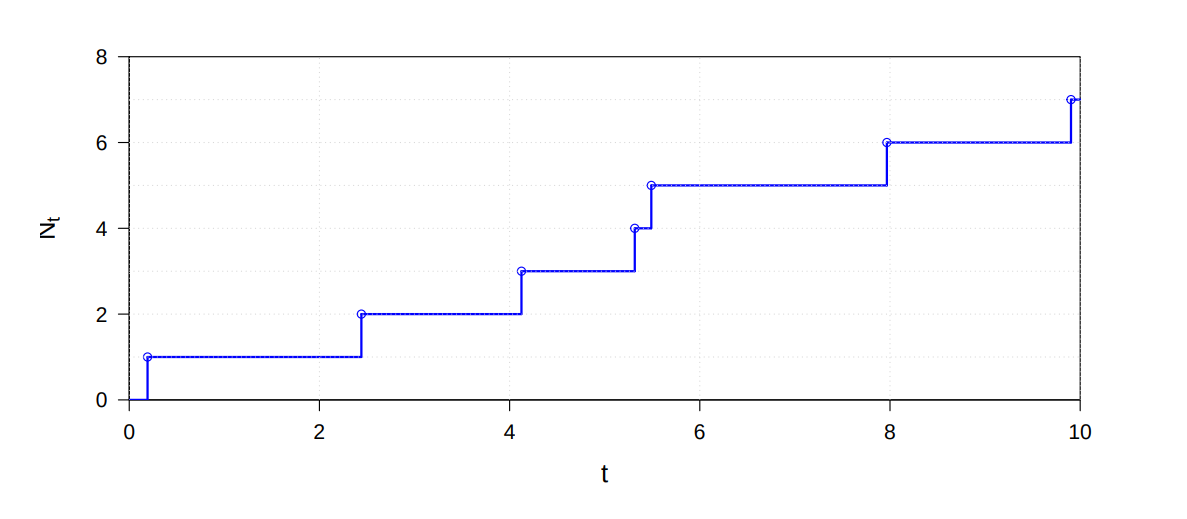
\includegraphics[width=\textwidth]{figures/sample_homogeneous_poisson_process.png}
    \caption{Homogeneous Poisson Process with constant jump size (figure sampled from \cite{book:privault})}
    \label{fig:sample-homogeneous-poisson-proc}
\end{figure}

\begin{proposition}{Properties of Poisson Process}{properties_of_poisson_proc}
    In order for the counting process $(N_t)_{t\ge0}$ to be a Poisson process, it has to satisfy the following properties:
    \begin{itemize}
        \item \textbf{Independence of increments} : For all $0 \le t_0 < t_1 < \dots < t_n$ and $n\ge1$ increments, we have
        \begin{align*}
            N_{t_1} - N_{t_0}, N_{t_2} - N_{t_1}, \dots, N_{t_n} - N_{t_{n-1}}
        \end{align*}
        \noindent are mutually independent random variables.
        \item \textbf{Stationarity of increments} : For all $0 \le s \le t$ and some $h>0$, the increment $N_{t} - N_s$ has the same distribution as $N_{t+h} - N_{s+h}$. In other words, for some $k\ge 0$, we have:
        \begin{align*}
            P(N_{t+h} - N_{s+h} = k) = P(N_t - N_s = k)
        \end{align*}
    \end{itemize}
\end{proposition}

\begin{theorem}{Poisson increment}{poisson_increment}
    Let $(N_t)_{t\ge0}$ be a Poisson process. For any $0 \le s \le t$, the increment $N_t-N_s$ follows a Poisson distribution with parameter $(t-s)\lambda$ for some $\lambda > 0$.
    \begin{align*}
        N_t - N_s \sim Poisson\Big( (t-s)\lambda \Big)
    \end{align*}

    \noindent The constant $\lambda$ is called the \textbf{intensity of Poisson process} $(N_t)_{t\ge0}$ and is given by:
    \begin{align*}
        \lambda = \lim_{h\to 0}\frac{1}{h}P(N_h=1)
    \end{align*}
    \noindent Intuitively, the parameter $\lambda$ reflects how soon it is the get the first count. The higher the intensity, the closer the gap in between jumps.
\end{theorem}
\begin{proof*}[Theorem \ref{thm:poisson_increment}]
    (The proof for theorem \ref{thm:poisson_increment} is too technical and will not be included. Refer to \cite{book:Bosq1996} for more information).
\end{proof*}

\begin{corollary}{Distribution of $N_t$}{distribution_of_nt}
    As a direct consequence of theorem \ref{thm:poisson_increment}, we have:
    \begin{align*}
        N_t\sim Poisson\Big( \lambda t \Big) \implies P(N_t = k) = \frac{(\lambda t)^ke^{-\lambda t}}{k!}
    \end{align*}
\end{corollary}

\begin{corollary}{Short-time asymptotics of Poisson process}{short_time_behaviour_poisson_proc}
    For a current state $N_t$ of the Poisson process, the behaviour of the process in a short time $h>0$ ahead is expressed in the following probability:
    \begin{align*}
        P(N_{t+h} - N_t) \approx \frac{\lambda^kh^k}{k!}, \ h \to 0
    \end{align*}
\end{corollary}
\begin{proof*}[Corollary \ref{coro:short_time_behaviour_poisson_proc}]
    By theorem \ref{thm:poisson_increment}, we have:
    \begin{align*}
        N_{t+h} - N_t \sim Poisson(h\lambda)
    \end{align*}

    \noindent Hence, we have:
    \begin{align*}
        P(N_{t+h} - N_t) &= \frac{(\lambda h)^k e^{-\lambda h}}{k!} \\
        &\approx \frac{\lambda^kh^k}{k!} \ \ \text{(When $h\approx 0$)}
    \end{align*}

    \noindent Because $e^{-\lambda h} \to 1$ as $h \to 0$.
\end{proof*}

\begin{proposition}{Distribution of jump-time $T_n$}{jump_time_distribution}
    For all $n\ge1$, the jump-time $T_n$ has the gamma distribution:
    \begin{align*}
        T_n \sim Gamma(n, 1/\lambda)
    \end{align*}

    \noindent With the probability density function:
    \begin{align*}
        f_{T_n}(t) = \lambda^n e^{-\lambda t}\frac{t^{n-1}}{(n-1)!} = \lambda^n e^{-\lambda t}\frac{t^{n-1}}{\Gamma(n)}
    \end{align*}
    \noindent For all $t>0$, the probability that $T_n\ge t$ is given by:
    \begin{align*}
        P(T_n \ge t) = \lambda^n \int_t^\infty e^{-\lambda s}\frac{s^{n-1}}{(n-1)!}ds
    \end{align*}
\end{proposition}
\begin{proof*}[Proposition \ref{prop:jump_time_distribution}]
    Proving by induction, for base case, we have:
    \begin{align*}
        P(T_1 \ge t) = P(T_1 > t) = P(N_t = 0) = e^{-\lambda t}
    \end{align*}

    \noindent For inductive case, suppose that we have:
    \begin{align*}
        P(T_{n-1} > t) = \lambda^{n-1}\int_{t}^{\infty} e^{-\lambda s}\frac{s^{n-2}}{(n-2)!}ds
    \end{align*}

    \noindent For $T_n$, we have:
    \begin{align*}
        P(T_n > t) &= P(T_n > t \ge T_{n-1}) + P(T_{n-1}>t) \\
        &= P(N_t = n-1) + P(T_{n-1} > t) \\
        &= \frac{(\lambda t)^{n-1} e^{-\lambda t}}{(n-1)!} + \lambda^{n-1}\int_{t}^{\infty} e^{-\lambda s}\frac{s^{n-2}}{(n-2)!}ds \\
        &= \lambda \int_{t}e^{-\lambda s}\frac{(\lambda s)^{n-1}}{(n-1)!}ds \\
        &= \lambda ^n\int_t^\infty \frac{e^{-\lambda s}s^{n-1}}{(n-1)!}ds
    \end{align*}
\end{proof*}

\subsection{Compound Poisson Process}
\begin{definition}[Compound Poisson Process]
    Let $(Z_k)_{k\ge1}$ be a sequence of i.i.d square integrable random variables with a probability distribution $\nu(.)$ independent of the Poisson Process $(N_t)_{t\ge0}$.

    \noindent\newline The process $(Y_t)_{t\ge0}$ is called a \textbf{Compound Poisson Process} if it is given by the random sum:
    \begin{align*}
        Y_t = \sum_{k=1}^{N_t}Z_k
    \end{align*}

    \noindent The Compound Poisson Process is indeed a Poisson process because it satisfies both properties:
    \begin{itemize}
        \item \textbf{Independent increments}.
        \item \textbf{Stationarity of increments}.
    \end{itemize}
\end{definition}

\begin{figure}[ht]
    \centering
    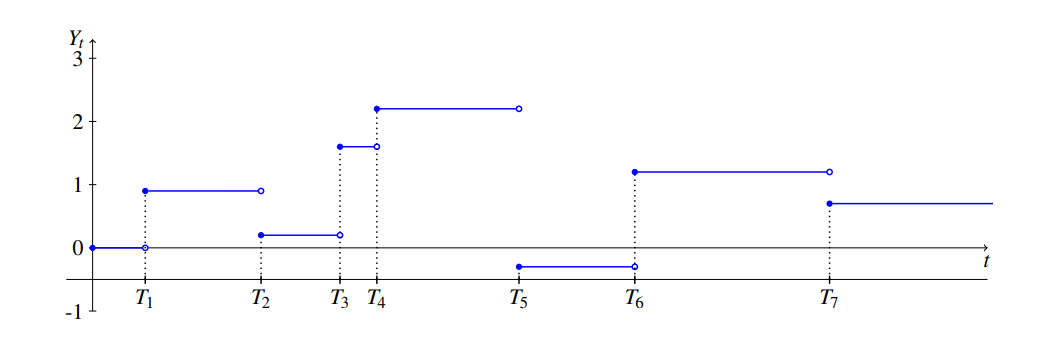
\includegraphics[width=\textwidth]{figures/sample_compound_poisson_process.png}
    \caption{Compound Poisson Process with non-constant jump size (figure sampled from \cite{book:privault})}
    \label{fig:sample-compound-poisson-process}
\end{figure}

\begin{proposition}{Mean and Variance of $(Y_t)_{t\ge0}$}{mean_var_of_comp_poisson_proc}
    Let $\mathbb{E}\Big[ N_t \Big]$ be the mean number of jump times and $\mathbb{E}\Big[Z\Big]$ be the mean jump size. We have:
    \begin{itemize}
        \item $\mathbb{E}[Y_t] = \mathbb{E}[N_t]\mathbb{E}[Z] = \lambda t\mathbb{E}[Z]$.
        \item $Var(Y_t) = \mathbb{E}[N_t] \mathbb{E}[Z^2] = \lambda t \mathbb{E}[Z^2]$.
    \end{itemize}
\end{proposition}

\subsection{Claim and Reserve Process}
\textbf{Overview} : In an insurance risk settings, we have
\begin{itemize}
    \item \textbf{Number of claims $(N_t)$} : modelled by the homogeneous (constant jump size) Poisson process $(N_t)_{t\ge0}$ with intensity $\lambda > 0$.
    \item \textbf{Claim amounts $(Z_k)$} : A sequence of non-negative, i.i.d random variables.
\end{itemize}

\begin{definition}[Aggregated claims]
    The \textbf{Aggregated claim} amount up to time $t$ is defined by the Compound Poisson Process:
    \begin{align*}
        S(t) = \sum_{k=1}^{N_t} Z_k
    \end{align*}
\end{definition}

\begin{definition}[Standard compound risk model]
    The reserve process is defined by
    \begin{align*}
        R_x(t) = x + f(t) - S(t)
    \end{align*}

    \noindent Where $x\ge0$ is the initial reserve, $f(t)$ is an income function up to time $t>0$ and $S(t)$ is the aggregated claims. 
\end{definition}

\begin{figure}[ht]
    \centering
    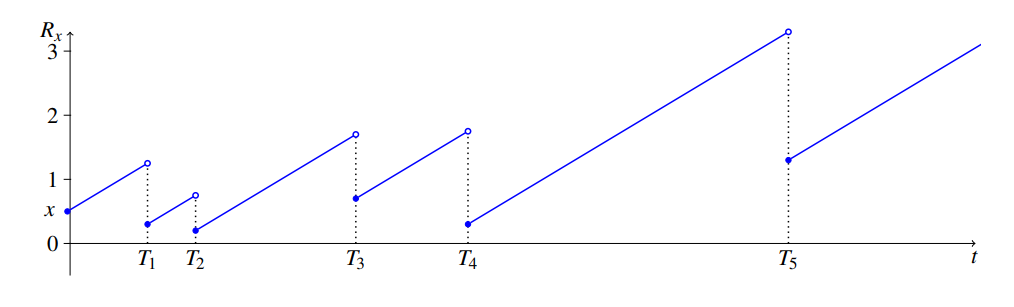
\includegraphics[width=\textwidth]{figures/sample_reserve_process.png}
    \caption{Sample reserve process with non-zero initial reserve and a linear income function (figure sampled from \cite{book:privault})}
    \label{fig:sample-reserve-process}
\end{figure}

\subsection{Ruin Probability}
\begin{definition}[Ruin probability]
    There are two types of ruin probabilities
    \begin{itemize}
        \item \textbf{Infinite-time ruin probability} :
        \begin{align*}
            \Psi(x) = P(\exists t \in [0, \infty) : R_x(t) < 0)
        \end{align*}

        \item \textbf{Finite-time ruin probability} :
        \begin{align*}
            \Psi_T(x) = P(\exists t \in [0, T]:R_x(t) < 0)
        \end{align*}
    \end{itemize}
\end{definition}

\begin{theorem}{Cramer Lundberg model}{cramer_lundberg}
    Assume that the income function is linear with a positive slope $f(t) = ct$. We have:
    \begin{itemize}
        \item \textbf{Zero initial reserve} : 
        \begin{align*}
            \Psi(x) = \frac{\lambda\mu}{c}
        \end{align*}
        \noindent Provided that $c > \lambda\mu$ where $\mu = \mathbb{E}[Z]$. 

        \item \textbf{Non-zero initial reserve} : Suppose that $Z_k \sim Exponential(1/\mu)$. then,
        \begin{align*}
            \Psi(x) = \frac{\lambda \mu}{c}\exp\Bigg(\Bigg( \frac{\lambda}{c} - \frac{1}{\mu} \Bigg)x\Bigg)
        \end{align*}
    \end{itemize}

    \noindent Either case, $\Psi(x)=1$ if $c \le \lambda \mu$.
\end{theorem}



%% Appendices %%
%% Start a new page %%
\newpage
\appendix

% List of Definitions
\listoftheorems[ignoreall,show=dfn]

% List of Theorems
\setcounter{section}{1}
\tcblistof[\section]{theoremlist}{Important Theorems}

% List of Corollaries
\tcblistof[\section]{corolist}{Important Corollaries}

% List of Propositions
\tcblistof[\section]{proplist}{Important Propositions}

% References
\newpage
\section{References}

% Commented as requested by Nicolas Privault, author of this course, to be more precise with references.
% \nocite{*}
\printbibliography

%% ========================================================================= %%
\end{document}
